% This must be in the first 5 lines to tell arXiv to use pdfLaTeX, which is strongly recommended.
\pdfoutput=1
% In particular, the hyperref package requires pdfLaTeX in order to break URLs across lines.

\documentclass[11pt]{article}

% Change "review" to "final" to generate the final (sometimes called camera-ready) version.
% Change to "preprint" to generate a non-anonymous version with page numbers.
\usepackage[review]{acl}
% Standard package includes
\usepackage{times}
\usepackage{latexsym}
\usepackage{graphicx}

\usepackage{algorithmic}
\usepackage{algorithm}
\usepackage{multirow}
\usepackage{natbib}
\usepackage{subcaption}

% For proper rendering and hyphenation of words containing Latin characters (including in bib files)
\usepackage[T1]{fontenc}
% For Vietnamese characters
% \usepackage[T5]{fontenc}
% See https://www.latex-project.org/help/documentation/encguide.pdf for other character sets

% This assumes your files are encoded as UTF8
\usepackage[utf8]{inputenc}
\usepackage[export]{adjustbox}

% This is not strictly necessary, and may be commented out,
% but it will improve the layout of the manuscript,
% and will typically save some space.
\usepackage{microtype}
\usepackage{hyperref}

% This is also not strictly necessary, and may be commented out.
% However, it will improve the aesthetics of text in
% the typewriter font.
\usepackage{inconsolata}
% If the title and author information does not fit in the area allocated, uncomment the following
%
%\setlength\titlebox{<dim>}
%
% and set <dim> to something 5cm or larger.
\newcommand{\secref}[1]{Sec. \ref{#1}}
\newcommand{\figref}[1]{Figure \ref{#1}}
\newcommand{\eqnref}[1]{Eq. (\ref{#1})}
\newcommand{\tabref}[1]{Table \ref{#1}}
\newcommand{\exref}[1]{Example \ref{#1}}
\newcommand{\ZZ}[1]{\textcolor{brown}{(Zander: #1})}
\newcommand{\KZ}[1]{\textcolor{blue}{(Kenny: #1})}
\newcommand{\MY}[1]{\textcolor{red}{(Mengyue: #1})}

\title{PersonaMovs: A Multimedia Conversational Dataset for Dynamic Personality Analysis}

% Author information can be set in various styles:
% For several authors from the same institution:
% \author{Author 1 \and ... \and Author n \\
%         Address line \\ ... \\ Address line}
% if the names do not fit well on one line use
%         Author 1 \\ {\bf Author 2} \\ ... \\ {\bf Author n} \\
% For authors from different institutions:
% \author{Author 1 \\ Address line \\  ... \\ Address line
%         \And  ... \And
%         Author n \\ Address line \\ ... \\ Address line}
% To start a separate ``row'' of authors use \AND, as in
% \author{Author 1 \\ Address line \\  ... \\ Address line
%         \AND
%         Author 2 \\ Address line \\ ... \\ Address line \And
%         Author 3 \\ Address line \\ ... \\ Address line}




\begin{document}
\maketitle
\begin{abstract}
Automatic personality detection has evolved from simple text classification to sophisticated multimodal analysis, recognizing the multidimensional manifestation of personality beyond textual data. This shift highlights the need for datasets that can accurately capture the complexity of human personality through diverse modalities. We introduce the PersonaMovs (PM), a large, extensive and varied multimedia conversational dataset, built on 305 movies and 14 TV series, featuring over 46k dialogues, 552k utterances, 4016 characters, and 963 hours of video. PM not only addresses the challenges of existing datasets by offering majority-voted personality annotations and detailed relations networks but also paves the way for advanced analysis of personality dynamics across various contexts.
\end{abstract}
%\IEEEraisesectionheading{
% %\IEEEraisesectionheading{
% %\IEEEraisesectionheading{
% \input{intro}
\section{Introduction}\label{sec:intro}
 %}
% \section{Introduction}\label{sec:intro}

% \begin{enumerate}
% \item Motivation: application scenarios (with 1-2 running examples);
% \item Characteristics of the data sources and their challenges;
% \item Briefly introduce previous approaches to extract information 
% from images including setting the document zone, and their limitations.
% \item General flow of our approach (may give a diagram here)
% \end{enumerate}
% scenary

Due to ever evolving hardware and software, many medical images
such as electro-cardio graphs (ECGs), X-ray or ultrasound images  
are directly printed and stored in hard copy formats. 
% \KZ{Insert 4 example images here.}
%Examples are shown in \figref{fig:medicalImages}. 
% These images often contain a mix of graphics and text, which
% include parameter settings of the hardware, test measurements or simple
% diagnosis. 
These images often contain a mix of graphics and text, which 
include technical settings of the hardware used, test measurements or simple diagnoses.
Recently, there has been a growing demand for digitizing such 
medical information from paper media sources, especially legacy ones, or patients who want to keep track of these documents by themselves digitally. 
Apart from scanning the graphics into a digital format, extracting 
the semi-structured textual information is also an important part of
building electronic medical records for patients. 

%\begin{figure}[!htb]
%\centering
%\subfloat[ECG]{
%\label{fig:medicalimage:ecg}
%\epsfig{file=figure/17_ori.eps, width=0.4\columnwidth}
%}
%% \hfill
%\subfloat[MRI]{
%	\label{fig:medicalimage:mrt}
%	\epsfig{file=figure/MRI.eps, width=0.4\columnwidth}
%}
%\\
%\subfloat[X-RAY]{
%\label{fig:medicalimage:xray}
%\epsfig{file=figure/X-RAY.eps, width=0.4\columnwidth}
%}
%%\hfill
%\subfloat[EEG]{
%\label{fig:medicalimage:eeg}
%\epsfig{file=figure/EEG.eps, width=0.4\columnwidth}
%}
%\caption{Examples of Medical Images}
%\label{fig:medicalImages}
%\end{figure}

Optical character recognition (OCR)  \cite{mori1992historical,smith2007overview} is 
a traditional technique used to turn images of printed text into machine encoded
text. It is well researched and performs well on plain text 
documents such as novels and reports, for a variety of languages. 
%For example, Tesseract, which is one of 
%the most popular open source multilingual recognizers, logs an error 
%rate of 3.72\% for English words and 3.77\% for simplified 
%Chinese characters\cite{smith2009adapting}. 
%Google Books \cite{googlebooks} and Gutenberg \cite{gutenberg} are
%projects which have scanned a large number of paper books into text for free and open
%access. These projects made exclusive use of OCR for this conversion and 
%achieved high accuracy \cite{vincent2007google} \cite{lebert2008project}. 
% 99\% for Gutenberg project \cite{lebert2008project}. 
% \KZ{Give the accuracy of google and gutenberg if available.}


\begin{figure}[th]
\centering
\epsfig{file=figure/17_b.eps, width=0.8\columnwidth}
\caption{An ECG image with text area (red circle) of interest.}
\label{fig:ecgexample2}
\end{figure}

For a semi-structured medical image, such as 
\figref{fig:ecgexample2}, we would like to extract the attribute-value 
pairs (e.g., {\em Vent. rate = 63 bpm}) and possibly other values such as
date ({\em 18-Nov-2010}) and time ({\em 9:13:02}) since those values endow us with lots of information about the patient. 
Existing OCR software cannot extract such structured information in a straightforward 
fashion, 
but instead it produces rather convoluted results from the whole image, 
similar to those in \figref{fig:ocrre}, which was produced by Tesseract, 
a popular multi-lingual recognizers. 
% \KZ{Maybe include the x-y coordinate info in the output as well?}  

\begin{figure}[th]
\centering
\scriptsize
\begin{verbatim}
<p class="ocr_par" title="box 263 33 444 119">
   <span class="ocr_l" title="box 264 33 336 45">
       <span class="ocrx_w" title="box 264 33 299 45">Vcnt.</span> 
       <span class="ocrx_w" title="box 308 34 336 45">rule</span> 
   </span>
   <span class='ocr_l'>
       <span class="ocrx_w" title="box 264 51 283 64">PR</span> 
       <span class="ocrx_w" title="box 291 51 346 64">Interval</span> 
       <span class="ocrx_w" title="box 389 52 411 64">140</span> 
       <span class="ocrx_w" title="box 420 55 439 64">ms</span> 
   </span>
   ...
   </span>
</p>
<p class="ocr_p" dir="ltr">
   <span class="ocr_l">
       <span class="ocrx_w" title="box 396 33 411 45">53</span> 
       <span class="ocrx_w" title="box 420 33 449 48">bpm</span> 
   </span>
</p>
\end{verbatim}
\caption{Snippet OCR results in XML, input to our framework.}
\label{fig:ocrre}
\end{figure}


%\input{xmlre1}

%However, OCR alone does not work well on semi-structured text and hence
%can't be directly used for information extraction from the aforementioned
%medical images. \KZ{Give the reason here, perhaps because OCR models are
%largely Markov based? So semi-structured data breaks the flow of text.}
%When a medical image is input to an ordinary OCR software, the spatial 
%information of the text components is often lost or mixed with noises
%and errors.
%%The reason is OCR converts the whole images into text data, in which 
%%useful information often mix with noises and errors. 
%In this paper, we would like to extract the attribute-value pairs
%and possibly other values from \figref{fig:ecgexample1} 
%and \figref{fig:ecgexample2}. 
%% or medical ultrasonography report. 
%Such images contain lots of non-textual information or noises.

% example & ref
%\begin{figure}[ht]
%\centering
%\epsfig{file=figure/46.eps, width=0.8\columnwidth}
%\caption{ECG Images From Printer1}
%\label{fig:ecgexample1}
%\end{figure}

% \begin{figure}[ht]
% \centering
% \subfloat[Printer1]{
% \label{fig:ecgexample:a}
% \epsfig{file=figure/46.eps, width=0.48\columnwidth}
% }
% \hfill
% \subfloat[Printer2]{
% \label{fig:ecgexample:b}
% \epsfig{file=figure/17.eps, width=0.48\columnwidth}
% }
% \caption{ECG images from two different printers}
% \label{fig:ecgexample}
% \end{figure}

Also, errors in the OCR text \cite{darwish2007error,taghva1996evaluation} will greatly affect the effectiveness 
of other related tasks. Much work has been done to improve the performance of the OCR\cite{kolak2003generative,cesarini1998informys}. However, there are still a number of significant challenges involved in extracting the information from medical images or OCR results in XML form. 

% First, medical images differ from pure text document in that them have 
% layout information. 
First, medical images differ from pure text documents in that 
they contain layout information.
Although most current OCR engines attempt to reproduce the physical 
layout of the text units, 
%(along with X-Y coordinates) and store them 
%in a special format such as XML 
% (\KZ{Better in the previous example})
such spatial
information is approximate and sometimes inaccurate, which is why neighboring
text blocks in \figref{fig:ecgexample2}, such as ``Vent. Rate'' and
``63 bpm'' were not automatically combined into the same XML block, but were 
rather far apart (shown in two different ``classes'') in \figref{fig:ocrre} made by OCR softwares. 
%Even for images produced by the same ECG printer, 
%the XML results can still be very different as 
The spatial layout is sensitive to many factors, such as accidental spots 
on the prints, color and contrast, or the angle of the camera. 
%In this case, solutions for other application domains, for example, the web, 
%are not well suited for information extraction from printed documents \cite{bartoli2014semisupervised}. With such inaccurate
%layout information produced by OCR,
%it is not easy to write a simple wrapper program to extract useful
%data from images, even if the images come from the same printer. 

%Writing a wrapper for each
%individual image would be tedious and counter-productive. Therefore,
%a mechanism that makes use of the spatial locality of the 
%text units in the image and 
%accommodates slight variations in the spatial layout would make the extraction
%more accurate and fault-tolerant.

%For example, \figref{fig:ocrre} is the simplified OCR results for the ECGs in 
%\figref{fig:ecgexample1} and \figref{fig:ecgexample2}. The results are in the XML format and have attritube named {\em class} 
%for layout information. Although these two images share similar format. 
%OCR engine generates different results in that it splits elements that 
%should be in the same line into two lines in the second example. 
%XML is sensitive to the layout results so it's hard to tolerate 
%all the layout results. 
%
% example check the term
% layout of ocr results can be restore, so why OCR engine don't restore the results 
% using the similar methods as we do?
% or the way we handle the layout problem is quite simple

% Delete for TIP
% Second, exiting OCR engines make heavy use of Markov properties such as n-grams
% since they primarily target the transformation of large body of text 
% \cite{kolak2003generative}. 
% % \KZ{Needs some refs here.}
% Unfortunately, the semi-structured texts in medical images are often 
% short and not even written in complete sentences, thus breaking Markov assumption. To make
% matters worse, medical images contain scientific language, which may be
% very different from the training corpora of these OCR engines.
% This explains why we see errors like ``Vcnt'' and ``rule'' 
% in \figref{fig:ocrre}. 
% %can't guarantee a perfect performance, which means 
% %there are errors and noises in the OCR results.
% %Many of them due to the fact that the data are no longer long, continous
% %sentences, thus breaking the Markov assumption made by many OCR algorithms. 
% %In \figref{fig:ocrresub:b}, ``Vent." is misrecognized as ``Vcnt.". 
% Without sufficient contextual information, OCR may also misrecognize a 
% digit as an alphabetic character, or as another similar digit. 
% Furthermore, the mix of text with images and formatting
% lines often confuses the OCR engine, which is more biased toward full
% text images.
% Exact pattern matching, as used in
% traditional information extraction, doesn't work with such noisy OCR output
% as it doesn't tolerate noises or errors in text. 
% %It's hard to autocorrect these errors 
% %because image quality is the most important affecting factor. 
% %The text we are processing can be full of no meaning words or 
% %strange numbers. 
% A fuzzy matching strategy is more desirable in this case. 
% % example, what are the traditional IEs

Second, there are many types of medical images, resulting from a variety of
medical tests. Different equipments for the same test can produce vastly 
different images. Writing individual extraction wrappers 
for the OCR outputs of all these formats is tedious and inefficient, 
and difficult for non-programmers.
%not to mention that there are significant programming barriers for 
%writing these wrappers, especially for the medical professionals who are the
%end users of these extraction results. 
%A more user-friendly approach enabling users to specify such extraction requirements would be preferred. 
%There are various kinds of medical images, such as electrocardiograph report, 
%medical ultrasonography report, etc. 
%However the basic measures for each type of medical test (e.g., ECG), 
%are very similar from machine to machine. Only the layouts are 
%different. 
% example medical images

Finally, most off-the-shelf OCR programs are pre-trained with specific 
recognition models, which may not be suitable for the extraction of 
%medical images.
%Furthermore, changes in imaging equipment technology over time may produce 
%different formats, layout, or terminology, rendering existing OCR models 
%obsolete. 
Re-training the models requires a large amount of labeled data, which may
not be available. 
%Incremental training as more labeled data arrives
%is currently not supported by any OCR product.    

%There have been some limited attempts to address some of the above challenges. 
%One solution is a plugin of an OCR program that allows the user to specify 
%target zones of interest in the image to be extracted. The zones specified for
%one image can be applied to images with slight variations by adjusting against
%a fixed reference point that is supposed to exist in all these images.
%% \KZ{I think the problem is not so much with the zones, because we also
%% have zones, but rather with the reference point.}
%% \JY{}
%% example products
%% http://www.square-9.com/automated-data-extraction-optical-character-recognition
%The problem with this solution is its high reliance on the OCR zones  
%established by the user. The performance of the results is affected by the 
%accuracy of the zones. If the zones are too big, the results will be full of 
%noise. If the zones are too small, results will miss something. 
%
%Another solution involves using the page layout analysis technique. The page layout 
%analysis technique is used to determine where the text 
%resides on a page \cite{o1993document}, 
%% \KZ{This page layout analysis approach is not clearly described. I don't understand after reading this paragraph.}
%% By using page layout analysis technique, the hierarchy of physical components 
%% can be generated and to match with the hierarchy of logical components, which 
%% is predefined. 
%this includes identifying and categorizing the 
%regions of interest in the scanned image of a text document. 
%Typically, the first step is to segment text zones from 
%non-textual zones and arrange them in their original order. 
%Then in order to analyze the logical roles of the text zones 
%(titles, captions, footnotes, etc.), logical layout analysis 
%is used for labeling the semantics of the text zones.
%Generally, page layout analysis is used for documents. The problem with applying 
%such a technique on medical images is that it creates so much noises 
%that performance is ultimately affected. 
%For medical imaging reports like ECG, useful information is often 
%found in the small components of the image, while most of the images are 
%read as noises. 
% check paper and more description, weakness, ref

%In this paper, 
%we propose a spatial data description language, which borrows its syntax from
%PADS \cite{fisher+:pads}, an ad hoc data processing language, 
%for describing semi-structured data in medical images. 
%% ref
%We call this language OCR description language, or ODL. 
%ODL is designed for extracting and parsing semi-structured text data 
%from images. We believe that  information extraction from those data in ODL form may be much easier than extracting information from rough data or data in XML form, which means that our preprocessing part proves to be necessary.
%%An example ODL description for the image in 
%%\figref{fig:ecgexample2} is shown in 
%%\figref{fig:description}. \KZ{Make this description two column, and give
%%some brief explanation of this description here.} 
%%The parsing result of this description is shown
%%in \figref{fig:parsing result}. \KZ{Give some explanation of the results,
%%otherwise don't show the result here. E.g., you need to explain what F, E, etc.
%%mean. You want to say that even though rate has been recognized as rule,
%%the bpm value was still extracted (but still wrong!).}
%% \KZ{I removed the preprocessing part, cos it's not important. Talk about it in
%% discussion sec.}
%%The our approach starts by preprocessing the images for text results.
%To use this framework, the user first describes the components in the image
%that he or she is interested in extracting. This includes constant strings
%and variables of different data types.   
%ODL allows the user to specify the approximate spatial layout and constraints on
%the data, e.g., integers within 
%a certain range, real numbers with certain decimal points, etc. 
%%This information is then as the key component in our fuzzy matching strategy. 
%The system then automatically generates a parser for these medical images.
%This parser uses the output XML from OCR with spatial information as an input, 
%and outputs a data structure with values extracted for each variables
%in the description, unless there is an unrecoverable error during the parsing process.
%In addition, approximate layout information and constraints are used in parsing process 
%to tolerate noises and small format variations in the input images. 
%%Specifically, this method could be called fuzzy matching, meaning that more candidates could be saved after the parsing process.  It's obvious that we may have a higher probability to obtain the accurate result if more candidates are kept so that fuzzy match should be used properly in our system.
%%An autogenerated parser based on the ODL description can release us from 
%%repetitive work. In this way, we turn the task of writing complex parsers 
%%into describing information on images.
%
%
%When users process many images of the same format, the system 
%automatically discovers parsing errors given the current model and 
%prompts the user to manually correct some of the frequent and prominent
%errors, which effectively serves as an online labeling function. 
%These incrementally labeled data are then used to update the parsing model. 


%It should be emphasized that the incremental learning model is very important in our whole system. Incremental learning is a machine learning paradigm where the learning process takes place whenever we have new examples or data added to our baisc data set, leading to a most striking difference between incremental learning and traditional machine learning: it does not assume the availability of a sufficient training set before the learning process. What incremental learning in our system is really impressive: it does not require a relatively good and stable training set at first time. In fact, it could improve the parsing result with even relatively rough training sets at first by absorbing new data or corrective information as time passes in dynamic systems. Besides, the process would be very effective when there are some new images coming in since training process would not learn from scratch, which might waste time and computation resource.

%At last, we propose an incrementally human correction framwork which can 
%make the best use of human correction to handle the misrecognition problem. 
% Base on our experiments on about 500 real life ECG images, 
% our approach achieves p1 and p2 after p3 times human correction. 
% experimental results

% \begin{figure}[h]
% \begin{lstlisting}
% Oenum str_month_t{
% 	"Jan", "Feb", "Mar", "Apr",
% 	"May", "Jun", "Jul", "Aug",
% 	"Sept", "Oct", "Nov", "Dec"
% };

% Ounion month_t{
% 	Oint(1,12)	num;
% 	str_month_t	str;
% };

% Ostruct time_t{
% 	Oint(1,31)	day;
% 	"-";
% 	month_t	month;
% 	"-";
% 	Oint	year;
% };

% Ostruct triple_t{
% 	"Vent.";
% 	hskip(\s)	skip1;
% 	"rate";
% 	Oint x;
% 	"bpm";
% 	vskip(\n)	skip2;
% };

% Oscource Ostruct entry_t{
% 	time_t(<-,-,-,0.3l>) t;
% 	triple_t(<0.1w,-,0.5w,->) d;
% };
% \end{lstlisting}
% \caption{Description}\label{fig:description}
% \end{figure}


In order to solve above problems, We design a system which makes three main contributions:
\begin{enumerate}
\item Based on some previous work on data description language \cite{lamport1986document,taft1999post,fisher+:pads},we design a new declarative spatial data description language called \textit{OCR description language}, or ODL,
which allows users to specify spatial and data constraints in medical 
images(\secref{sec:syntax});
\item We propose a noise-tolerant parser which takes OCR results
the ODL description as input and outputs a data structure with values 
extracted for each variables in the description (\secref{sec:semantics});
\item We propose an incremental manual correction 
framework\cite{von2008recaptcha,zhu2012learnpads++}, which 
takes advantage of user corrections  and improves the productivity
significantly (\secref{sec:correction}).
%To be more specific, the framework improves the traditional machine learning methods by using a incremental learning process to avoid starting from scratch when we are trying to apply human corrections in the system. That means the framework would be more effective than most corrective systems.
\end{enumerate}


\section{Introduction}\label{sec:intro}
 %}
% \section{Introduction}\label{sec:intro}

% \begin{enumerate}
% \item Motivation: application scenarios (with 1-2 running examples);
% \item Characteristics of the data sources and their challenges;
% \item Briefly introduce previous approaches to extract information 
% from images including setting the document zone, and their limitations.
% \item General flow of our approach (may give a diagram here)
% \end{enumerate}
% scenary

Due to ever evolving hardware and software, many medical images
such as electro-cardio graphs (ECGs), X-ray or ultrasound images  
are directly printed and stored in hard copy formats. 
% \KZ{Insert 4 example images here.}
%Examples are shown in \figref{fig:medicalImages}. 
% These images often contain a mix of graphics and text, which
% include parameter settings of the hardware, test measurements or simple
% diagnosis. 
These images often contain a mix of graphics and text, which 
include technical settings of the hardware used, test measurements or simple diagnoses.
Recently, there has been a growing demand for digitizing such 
medical information from paper media sources, especially legacy ones, or patients who want to keep track of these documents by themselves digitally. 
Apart from scanning the graphics into a digital format, extracting 
the semi-structured textual information is also an important part of
building electronic medical records for patients. 

%\begin{figure}[!htb]
%\centering
%\subfloat[ECG]{
%\label{fig:medicalimage:ecg}
%\epsfig{file=figure/17_ori.eps, width=0.4\columnwidth}
%}
%% \hfill
%\subfloat[MRI]{
%	\label{fig:medicalimage:mrt}
%	\epsfig{file=figure/MRI.eps, width=0.4\columnwidth}
%}
%\\
%\subfloat[X-RAY]{
%\label{fig:medicalimage:xray}
%\epsfig{file=figure/X-RAY.eps, width=0.4\columnwidth}
%}
%%\hfill
%\subfloat[EEG]{
%\label{fig:medicalimage:eeg}
%\epsfig{file=figure/EEG.eps, width=0.4\columnwidth}
%}
%\caption{Examples of Medical Images}
%\label{fig:medicalImages}
%\end{figure}

Optical character recognition (OCR)  \cite{mori1992historical,smith2007overview} is 
a traditional technique used to turn images of printed text into machine encoded
text. It is well researched and performs well on plain text 
documents such as novels and reports, for a variety of languages. 
%For example, Tesseract, which is one of 
%the most popular open source multilingual recognizers, logs an error 
%rate of 3.72\% for English words and 3.77\% for simplified 
%Chinese characters\cite{smith2009adapting}. 
%Google Books \cite{googlebooks} and Gutenberg \cite{gutenberg} are
%projects which have scanned a large number of paper books into text for free and open
%access. These projects made exclusive use of OCR for this conversion and 
%achieved high accuracy \cite{vincent2007google} \cite{lebert2008project}. 
% 99\% for Gutenberg project \cite{lebert2008project}. 
% \KZ{Give the accuracy of google and gutenberg if available.}


\begin{figure}[th]
\centering
\epsfig{file=figure/17_b.eps, width=0.8\columnwidth}
\caption{An ECG image with text area (red circle) of interest.}
\label{fig:ecgexample2}
\end{figure}

For a semi-structured medical image, such as 
\figref{fig:ecgexample2}, we would like to extract the attribute-value 
pairs (e.g., {\em Vent. rate = 63 bpm}) and possibly other values such as
date ({\em 18-Nov-2010}) and time ({\em 9:13:02}) since those values endow us with lots of information about the patient. 
Existing OCR software cannot extract such structured information in a straightforward 
fashion, 
but instead it produces rather convoluted results from the whole image, 
similar to those in \figref{fig:ocrre}, which was produced by Tesseract, 
a popular multi-lingual recognizers. 
% \KZ{Maybe include the x-y coordinate info in the output as well?}  

\begin{figure}[th]
\centering
\scriptsize
\begin{verbatim}
<p class="ocr_par" title="box 263 33 444 119">
   <span class="ocr_l" title="box 264 33 336 45">
       <span class="ocrx_w" title="box 264 33 299 45">Vcnt.</span> 
       <span class="ocrx_w" title="box 308 34 336 45">rule</span> 
   </span>
   <span class='ocr_l'>
       <span class="ocrx_w" title="box 264 51 283 64">PR</span> 
       <span class="ocrx_w" title="box 291 51 346 64">Interval</span> 
       <span class="ocrx_w" title="box 389 52 411 64">140</span> 
       <span class="ocrx_w" title="box 420 55 439 64">ms</span> 
   </span>
   ...
   </span>
</p>
<p class="ocr_p" dir="ltr">
   <span class="ocr_l">
       <span class="ocrx_w" title="box 396 33 411 45">53</span> 
       <span class="ocrx_w" title="box 420 33 449 48">bpm</span> 
   </span>
</p>
\end{verbatim}
\caption{Snippet OCR results in XML, input to our framework.}
\label{fig:ocrre}
\end{figure}


%% \begin{figure}[ht]
% \centering
% \subfigure[]{
% \label{fig:subfig:a}
% \begin{minipage}[b]{0.2\textwidth}
%\newsavebox{\firstlisting}
%\begin{lrbox}{\firstlisting}% Store first listing
%\begin{lstlisting}
%<p class='ocr_par' dir='ltr'>
%   <span class='ocr_line' id='line_2'>
%       <span class='ocrx_word' id='word_6'>Vent.</span>
%       <span class='ocrx_word' id='word_7'>rate</span>
%       <span class='ocrx_word' id='word_8'>65</span>
%       <span class='ocrx_word' id='word_9'>bpm</span>
%   </span>
%   <span class='ocr_line' id='line_3'>
%       <span class='ocrx_word' id='word_14'>PR</span>
%       <span class='ocrx_word' id='word_15'>interval</span>
%       <span class='ocrx_word' id='word_16'>162</span>
%       <span class='ocrx_word' id='word_17'>ms</span>
%   </span>
%    ...
%</p>
%\end{lstlisting}
%\end{lrbox}
% \end{minipage}
% }
% \hspace[1in]
% \subfigure[]{
% % \label{fig:subfig:b}
% % \begin{minipage}[b]{0.2\textwidth}
\newsavebox{\secondlisting}
\begin{lrbox}{\secondlisting}
% \tiny
\begin{lstlisting}[basicstyle=\tiny,]
<p class="ocr_par" title="box 263 33 444 119">
   <span class="ocr_l" title="box 264 33 336 45">
       <span class="ocrx_w" title="box 264 33 299 45">Vcnt.</span>
       <span class="ocrx_w" title="box 308 34 336 45">rule</span>
   </span>
   <span class='ocr_l'>
       <span class="ocrx_w" title="box 264 51 283 64">PR</span>
       <span class="ocrx_w" title="box 291 51 346 64">Interval</span>
       <span class="ocrx_w" title="box 389 52 411 64">140</span>
       <span class="ocrx_w" title="box 420 55 439 64">ms</span>
   </span>
   ...
   </span>
</p>
<p class="ocr_p" dir="ltr">
   <span class="ocr_l">
       <span class="ocrx_w" title="box 396 33 411 45">53</span>
       <span class="ocrx_w" title="box 420 33 449 48">bpm</span>
   </span>
</p>
\end{lstlisting}
\end{lrbox}
% % \end{minipage}
% }

% \KZ{\figref{fig:ocrre} is output from what software? Tesseract?}
\begin{figure*}[th]
%\subfloat[Image From Printer1]{
%\label{fig:ocrresub:a}
%\scalebox{0.8}{\usebox{\firstlisting}}}
%\hfill
%\subfloat[Image From Printer2]{
\scalebox{1.6}{\usebox{\secondlisting}}
% \label{fig:ocrre}
\caption{A fragment of raw OCR results for ECG with layout information.}
%\caption{Simplified OCR Results in XML for an ECG with Layout Information}
%\label{fig:ocrresub:b}
\label{fig:running-xml}
\end{figure*}

% \lipsum[2]


%However, OCR alone does not work well on semi-structured text and hence
%can't be directly used for information extraction from the aforementioned
%medical images. \KZ{Give the reason here, perhaps because OCR models are
%largely Markov based? So semi-structured data breaks the flow of text.}
%When a medical image is input to an ordinary OCR software, the spatial 
%information of the text components is often lost or mixed with noises
%and errors.
%%The reason is OCR converts the whole images into text data, in which 
%%useful information often mix with noises and errors. 
%In this paper, we would like to extract the attribute-value pairs
%and possibly other values from \figref{fig:ecgexample1} 
%and \figref{fig:ecgexample2}. 
%% or medical ultrasonography report. 
%Such images contain lots of non-textual information or noises.

% example & ref
%\begin{figure}[ht]
%\centering
%\epsfig{file=figure/46.eps, width=0.8\columnwidth}
%\caption{ECG Images From Printer1}
%\label{fig:ecgexample1}
%\end{figure}

% \begin{figure}[ht]
% \centering
% \subfloat[Printer1]{
% \label{fig:ecgexample:a}
% \epsfig{file=figure/46.eps, width=0.48\columnwidth}
% }
% \hfill
% \subfloat[Printer2]{
% \label{fig:ecgexample:b}
% \epsfig{file=figure/17.eps, width=0.48\columnwidth}
% }
% \caption{ECG images from two different printers}
% \label{fig:ecgexample}
% \end{figure}

Also, errors in the OCR text \cite{darwish2007error,taghva1996evaluation} will greatly affect the effectiveness 
of other related tasks. Much work has been done to improve the performance of the OCR\cite{kolak2003generative,cesarini1998informys}. However, there are still a number of significant challenges involved in extracting the information from medical images or OCR results in XML form. 

% First, medical images differ from pure text document in that them have 
% layout information. 
First, medical images differ from pure text documents in that 
they contain layout information.
Although most current OCR engines attempt to reproduce the physical 
layout of the text units, 
%(along with X-Y coordinates) and store them 
%in a special format such as XML 
% (\KZ{Better in the previous example})
such spatial
information is approximate and sometimes inaccurate, which is why neighboring
text blocks in \figref{fig:ecgexample2}, such as ``Vent. Rate'' and
``63 bpm'' were not automatically combined into the same XML block, but were 
rather far apart (shown in two different ``classes'') in \figref{fig:ocrre} made by OCR softwares. 
%Even for images produced by the same ECG printer, 
%the XML results can still be very different as 
The spatial layout is sensitive to many factors, such as accidental spots 
on the prints, color and contrast, or the angle of the camera. 
%In this case, solutions for other application domains, for example, the web, 
%are not well suited for information extraction from printed documents \cite{bartoli2014semisupervised}. With such inaccurate
%layout information produced by OCR,
%it is not easy to write a simple wrapper program to extract useful
%data from images, even if the images come from the same printer. 

%Writing a wrapper for each
%individual image would be tedious and counter-productive. Therefore,
%a mechanism that makes use of the spatial locality of the 
%text units in the image and 
%accommodates slight variations in the spatial layout would make the extraction
%more accurate and fault-tolerant.

%For example, \figref{fig:ocrre} is the simplified OCR results for the ECGs in 
%\figref{fig:ecgexample1} and \figref{fig:ecgexample2}. The results are in the XML format and have attritube named {\em class} 
%for layout information. Although these two images share similar format. 
%OCR engine generates different results in that it splits elements that 
%should be in the same line into two lines in the second example. 
%XML is sensitive to the layout results so it's hard to tolerate 
%all the layout results. 
%
% example check the term
% layout of ocr results can be restore, so why OCR engine don't restore the results 
% using the similar methods as we do?
% or the way we handle the layout problem is quite simple

% Delete for TIP
% Second, exiting OCR engines make heavy use of Markov properties such as n-grams
% since they primarily target the transformation of large body of text 
% \cite{kolak2003generative}. 
% % \KZ{Needs some refs here.}
% Unfortunately, the semi-structured texts in medical images are often 
% short and not even written in complete sentences, thus breaking Markov assumption. To make
% matters worse, medical images contain scientific language, which may be
% very different from the training corpora of these OCR engines.
% This explains why we see errors like ``Vcnt'' and ``rule'' 
% in \figref{fig:ocrre}. 
% %can't guarantee a perfect performance, which means 
% %there are errors and noises in the OCR results.
% %Many of them due to the fact that the data are no longer long, continous
% %sentences, thus breaking the Markov assumption made by many OCR algorithms. 
% %In \figref{fig:ocrresub:b}, ``Vent." is misrecognized as ``Vcnt.". 
% Without sufficient contextual information, OCR may also misrecognize a 
% digit as an alphabetic character, or as another similar digit. 
% Furthermore, the mix of text with images and formatting
% lines often confuses the OCR engine, which is more biased toward full
% text images.
% Exact pattern matching, as used in
% traditional information extraction, doesn't work with such noisy OCR output
% as it doesn't tolerate noises or errors in text. 
% %It's hard to autocorrect these errors 
% %because image quality is the most important affecting factor. 
% %The text we are processing can be full of no meaning words or 
% %strange numbers. 
% A fuzzy matching strategy is more desirable in this case. 
% % example, what are the traditional IEs

Second, there are many types of medical images, resulting from a variety of
medical tests. Different equipments for the same test can produce vastly 
different images. Writing individual extraction wrappers 
for the OCR outputs of all these formats is tedious and inefficient, 
and difficult for non-programmers.
%not to mention that there are significant programming barriers for 
%writing these wrappers, especially for the medical professionals who are the
%end users of these extraction results. 
%A more user-friendly approach enabling users to specify such extraction requirements would be preferred. 
%There are various kinds of medical images, such as electrocardiograph report, 
%medical ultrasonography report, etc. 
%However the basic measures for each type of medical test (e.g., ECG), 
%are very similar from machine to machine. Only the layouts are 
%different. 
% example medical images

Finally, most off-the-shelf OCR programs are pre-trained with specific 
recognition models, which may not be suitable for the extraction of 
%medical images.
%Furthermore, changes in imaging equipment technology over time may produce 
%different formats, layout, or terminology, rendering existing OCR models 
%obsolete. 
Re-training the models requires a large amount of labeled data, which may
not be available. 
%Incremental training as more labeled data arrives
%is currently not supported by any OCR product.    

%There have been some limited attempts to address some of the above challenges. 
%One solution is a plugin of an OCR program that allows the user to specify 
%target zones of interest in the image to be extracted. The zones specified for
%one image can be applied to images with slight variations by adjusting against
%a fixed reference point that is supposed to exist in all these images.
%% \KZ{I think the problem is not so much with the zones, because we also
%% have zones, but rather with the reference point.}
%% \JY{}
%% example products
%% http://www.square-9.com/automated-data-extraction-optical-character-recognition
%The problem with this solution is its high reliance on the OCR zones  
%established by the user. The performance of the results is affected by the 
%accuracy of the zones. If the zones are too big, the results will be full of 
%noise. If the zones are too small, results will miss something. 
%
%Another solution involves using the page layout analysis technique. The page layout 
%analysis technique is used to determine where the text 
%resides on a page \cite{o1993document}, 
%% \KZ{This page layout analysis approach is not clearly described. I don't understand after reading this paragraph.}
%% By using page layout analysis technique, the hierarchy of physical components 
%% can be generated and to match with the hierarchy of logical components, which 
%% is predefined. 
%this includes identifying and categorizing the 
%regions of interest in the scanned image of a text document. 
%Typically, the first step is to segment text zones from 
%non-textual zones and arrange them in their original order. 
%Then in order to analyze the logical roles of the text zones 
%(titles, captions, footnotes, etc.), logical layout analysis 
%is used for labeling the semantics of the text zones.
%Generally, page layout analysis is used for documents. The problem with applying 
%such a technique on medical images is that it creates so much noises 
%that performance is ultimately affected. 
%For medical imaging reports like ECG, useful information is often 
%found in the small components of the image, while most of the images are 
%read as noises. 
% check paper and more description, weakness, ref

%In this paper, 
%we propose a spatial data description language, which borrows its syntax from
%PADS \cite{fisher+:pads}, an ad hoc data processing language, 
%for describing semi-structured data in medical images. 
%% ref
%We call this language OCR description language, or ODL. 
%ODL is designed for extracting and parsing semi-structured text data 
%from images. We believe that  information extraction from those data in ODL form may be much easier than extracting information from rough data or data in XML form, which means that our preprocessing part proves to be necessary.
%%An example ODL description for the image in 
%%\figref{fig:ecgexample2} is shown in 
%%\figref{fig:description}. \KZ{Make this description two column, and give
%%some brief explanation of this description here.} 
%%The parsing result of this description is shown
%%in \figref{fig:parsing result}. \KZ{Give some explanation of the results,
%%otherwise don't show the result here. E.g., you need to explain what F, E, etc.
%%mean. You want to say that even though rate has been recognized as rule,
%%the bpm value was still extracted (but still wrong!).}
%% \KZ{I removed the preprocessing part, cos it's not important. Talk about it in
%% discussion sec.}
%%The our approach starts by preprocessing the images for text results.
%To use this framework, the user first describes the components in the image
%that he or she is interested in extracting. This includes constant strings
%and variables of different data types.   
%ODL allows the user to specify the approximate spatial layout and constraints on
%the data, e.g., integers within 
%a certain range, real numbers with certain decimal points, etc. 
%%This information is then as the key component in our fuzzy matching strategy. 
%The system then automatically generates a parser for these medical images.
%This parser uses the output XML from OCR with spatial information as an input, 
%and outputs a data structure with values extracted for each variables
%in the description, unless there is an unrecoverable error during the parsing process.
%In addition, approximate layout information and constraints are used in parsing process 
%to tolerate noises and small format variations in the input images. 
%%Specifically, this method could be called fuzzy matching, meaning that more candidates could be saved after the parsing process.  It's obvious that we may have a higher probability to obtain the accurate result if more candidates are kept so that fuzzy match should be used properly in our system.
%%An autogenerated parser based on the ODL description can release us from 
%%repetitive work. In this way, we turn the task of writing complex parsers 
%%into describing information on images.
%
%
%When users process many images of the same format, the system 
%automatically discovers parsing errors given the current model and 
%prompts the user to manually correct some of the frequent and prominent
%errors, which effectively serves as an online labeling function. 
%These incrementally labeled data are then used to update the parsing model. 


%It should be emphasized that the incremental learning model is very important in our whole system. Incremental learning is a machine learning paradigm where the learning process takes place whenever we have new examples or data added to our baisc data set, leading to a most striking difference between incremental learning and traditional machine learning: it does not assume the availability of a sufficient training set before the learning process. What incremental learning in our system is really impressive: it does not require a relatively good and stable training set at first time. In fact, it could improve the parsing result with even relatively rough training sets at first by absorbing new data or corrective information as time passes in dynamic systems. Besides, the process would be very effective when there are some new images coming in since training process would not learn from scratch, which might waste time and computation resource.

%At last, we propose an incrementally human correction framwork which can 
%make the best use of human correction to handle the misrecognition problem. 
% Base on our experiments on about 500 real life ECG images, 
% our approach achieves p1 and p2 after p3 times human correction. 
% experimental results

% \begin{figure}[h]
% \begin{lstlisting}
% Oenum str_month_t{
% 	"Jan", "Feb", "Mar", "Apr",
% 	"May", "Jun", "Jul", "Aug",
% 	"Sept", "Oct", "Nov", "Dec"
% };

% Ounion month_t{
% 	Oint(1,12)	num;
% 	str_month_t	str;
% };

% Ostruct time_t{
% 	Oint(1,31)	day;
% 	"-";
% 	month_t	month;
% 	"-";
% 	Oint	year;
% };

% Ostruct triple_t{
% 	"Vent.";
% 	hskip(\s)	skip1;
% 	"rate";
% 	Oint x;
% 	"bpm";
% 	vskip(\n)	skip2;
% };

% Oscource Ostruct entry_t{
% 	time_t(<-,-,-,0.3l>) t;
% 	triple_t(<0.1w,-,0.5w,->) d;
% };
% \end{lstlisting}
% \caption{Description}\label{fig:description}
% \end{figure}


In order to solve above problems, We design a system which makes three main contributions:
\begin{enumerate}
\item Based on some previous work on data description language \cite{lamport1986document,taft1999post,fisher+:pads},we design a new declarative spatial data description language called \textit{OCR description language}, or ODL,
which allows users to specify spatial and data constraints in medical 
images(\secref{sec:syntax});
\item We propose a noise-tolerant parser which takes OCR results
the ODL description as input and outputs a data structure with values 
extracted for each variables in the description (\secref{sec:semantics});
\item We propose an incremental manual correction 
framework\cite{von2008recaptcha,zhu2012learnpads++}, which 
takes advantage of user corrections  and improves the productivity
significantly (\secref{sec:correction}).
%To be more specific, the framework improves the traditional machine learning methods by using a incremental learning process to avoid starting from scratch when we are trying to apply human corrections in the system. That means the framework would be more effective than most corrective systems.
\end{enumerate}


\section{Introduction}\label{sec:intro}
 %}
% \section{Introduction}\label{sec:intro}

% \begin{enumerate}
% \item Motivation: application scenarios (with 1-2 running examples);
% \item Characteristics of the data sources and their challenges;
% \item Briefly introduce previous approaches to extract information 
% from images including setting the document zone, and their limitations.
% \item General flow of our approach (may give a diagram here)
% \end{enumerate}
% scenary

Due to ever evolving hardware and software, many medical images
such as electro-cardio graphs (ECGs), X-ray or ultrasound images  
are directly printed and stored in hard copy formats. 
% \KZ{Insert 4 example images here.}
%Examples are shown in \figref{fig:medicalImages}. 
% These images often contain a mix of graphics and text, which
% include parameter settings of the hardware, test measurements or simple
% diagnosis. 
These images often contain a mix of graphics and text, which 
include technical settings of the hardware used, test measurements or simple diagnoses.
Recently, there has been a growing demand for digitizing such 
medical information from paper media sources, especially legacy ones, or patients who want to keep track of these documents by themselves digitally. 
Apart from scanning the graphics into a digital format, extracting 
the semi-structured textual information is also an important part of
building electronic medical records for patients. 

%\begin{figure}[!htb]
%\centering
%\subfloat[ECG]{
%\label{fig:medicalimage:ecg}
%\epsfig{file=figure/17_ori.eps, width=0.4\columnwidth}
%}
%% \hfill
%\subfloat[MRI]{
%	\label{fig:medicalimage:mrt}
%	\epsfig{file=figure/MRI.eps, width=0.4\columnwidth}
%}
%\\
%\subfloat[X-RAY]{
%\label{fig:medicalimage:xray}
%\epsfig{file=figure/X-RAY.eps, width=0.4\columnwidth}
%}
%%\hfill
%\subfloat[EEG]{
%\label{fig:medicalimage:eeg}
%\epsfig{file=figure/EEG.eps, width=0.4\columnwidth}
%}
%\caption{Examples of Medical Images}
%\label{fig:medicalImages}
%\end{figure}

Optical character recognition (OCR)  \cite{mori1992historical,smith2007overview} is 
a traditional technique used to turn images of printed text into machine encoded
text. It is well researched and performs well on plain text 
documents such as novels and reports, for a variety of languages. 
%For example, Tesseract, which is one of 
%the most popular open source multilingual recognizers, logs an error 
%rate of 3.72\% for English words and 3.77\% for simplified 
%Chinese characters\cite{smith2009adapting}. 
%Google Books \cite{googlebooks} and Gutenberg \cite{gutenberg} are
%projects which have scanned a large number of paper books into text for free and open
%access. These projects made exclusive use of OCR for this conversion and 
%achieved high accuracy \cite{vincent2007google} \cite{lebert2008project}. 
% 99\% for Gutenberg project \cite{lebert2008project}. 
% \KZ{Give the accuracy of google and gutenberg if available.}


\begin{figure}[th]
\centering
\epsfig{file=figure/17_b.eps, width=0.8\columnwidth}
\caption{An ECG image with text area (red circle) of interest.}
\label{fig:ecgexample2}
\end{figure}

For a semi-structured medical image, such as 
\figref{fig:ecgexample2}, we would like to extract the attribute-value 
pairs (e.g., {\em Vent. rate = 63 bpm}) and possibly other values such as
date ({\em 18-Nov-2010}) and time ({\em 9:13:02}) since those values endow us with lots of information about the patient. 
Existing OCR software cannot extract such structured information in a straightforward 
fashion, 
but instead it produces rather convoluted results from the whole image, 
similar to those in \figref{fig:ocrre}, which was produced by Tesseract, 
a popular multi-lingual recognizers. 
% \KZ{Maybe include the x-y coordinate info in the output as well?}  

\begin{figure}[th]
\centering
\scriptsize
\begin{verbatim}
<p class="ocr_par" title="box 263 33 444 119">
   <span class="ocr_l" title="box 264 33 336 45">
       <span class="ocrx_w" title="box 264 33 299 45">Vcnt.</span> 
       <span class="ocrx_w" title="box 308 34 336 45">rule</span> 
   </span>
   <span class='ocr_l'>
       <span class="ocrx_w" title="box 264 51 283 64">PR</span> 
       <span class="ocrx_w" title="box 291 51 346 64">Interval</span> 
       <span class="ocrx_w" title="box 389 52 411 64">140</span> 
       <span class="ocrx_w" title="box 420 55 439 64">ms</span> 
   </span>
   ...
   </span>
</p>
<p class="ocr_p" dir="ltr">
   <span class="ocr_l">
       <span class="ocrx_w" title="box 396 33 411 45">53</span> 
       <span class="ocrx_w" title="box 420 33 449 48">bpm</span> 
   </span>
</p>
\end{verbatim}
\caption{Snippet OCR results in XML, input to our framework.}
\label{fig:ocrre}
\end{figure}


%% \begin{figure}[ht]
% \centering
% \subfigure[]{
% \label{fig:subfig:a}
% \begin{minipage}[b]{0.2\textwidth}
%\newsavebox{\firstlisting}
%\begin{lrbox}{\firstlisting}% Store first listing
%\begin{lstlisting}
%<p class='ocr_par' dir='ltr'>
%   <span class='ocr_line' id='line_2'>
%       <span class='ocrx_word' id='word_6'>Vent.</span>
%       <span class='ocrx_word' id='word_7'>rate</span>
%       <span class='ocrx_word' id='word_8'>65</span>
%       <span class='ocrx_word' id='word_9'>bpm</span>
%   </span>
%   <span class='ocr_line' id='line_3'>
%       <span class='ocrx_word' id='word_14'>PR</span>
%       <span class='ocrx_word' id='word_15'>interval</span>
%       <span class='ocrx_word' id='word_16'>162</span>
%       <span class='ocrx_word' id='word_17'>ms</span>
%   </span>
%    ...
%</p>
%\end{lstlisting}
%\end{lrbox}
% \end{minipage}
% }
% \hspace[1in]
% \subfigure[]{
% % \label{fig:subfig:b}
% % \begin{minipage}[b]{0.2\textwidth}
\newsavebox{\secondlisting}
\begin{lrbox}{\secondlisting}
% \tiny
\begin{lstlisting}[basicstyle=\tiny,]
<p class="ocr_par" title="box 263 33 444 119">
   <span class="ocr_l" title="box 264 33 336 45">
       <span class="ocrx_w" title="box 264 33 299 45">Vcnt.</span>
       <span class="ocrx_w" title="box 308 34 336 45">rule</span>
   </span>
   <span class='ocr_l'>
       <span class="ocrx_w" title="box 264 51 283 64">PR</span>
       <span class="ocrx_w" title="box 291 51 346 64">Interval</span>
       <span class="ocrx_w" title="box 389 52 411 64">140</span>
       <span class="ocrx_w" title="box 420 55 439 64">ms</span>
   </span>
   ...
   </span>
</p>
<p class="ocr_p" dir="ltr">
   <span class="ocr_l">
       <span class="ocrx_w" title="box 396 33 411 45">53</span>
       <span class="ocrx_w" title="box 420 33 449 48">bpm</span>
   </span>
</p>
\end{lstlisting}
\end{lrbox}
% % \end{minipage}
% }

% \KZ{\figref{fig:ocrre} is output from what software? Tesseract?}
\begin{figure*}[th]
%\subfloat[Image From Printer1]{
%\label{fig:ocrresub:a}
%\scalebox{0.8}{\usebox{\firstlisting}}}
%\hfill
%\subfloat[Image From Printer2]{
\scalebox{1.6}{\usebox{\secondlisting}}
% \label{fig:ocrre}
\caption{A fragment of raw OCR results for ECG with layout information.}
%\caption{Simplified OCR Results in XML for an ECG with Layout Information}
%\label{fig:ocrresub:b}
\label{fig:running-xml}
\end{figure*}

% \lipsum[2]


%However, OCR alone does not work well on semi-structured text and hence
%can't be directly used for information extraction from the aforementioned
%medical images. \KZ{Give the reason here, perhaps because OCR models are
%largely Markov based? So semi-structured data breaks the flow of text.}
%When a medical image is input to an ordinary OCR software, the spatial 
%information of the text components is often lost or mixed with noises
%and errors.
%%The reason is OCR converts the whole images into text data, in which 
%%useful information often mix with noises and errors. 
%In this paper, we would like to extract the attribute-value pairs
%and possibly other values from \figref{fig:ecgexample1} 
%and \figref{fig:ecgexample2}. 
%% or medical ultrasonography report. 
%Such images contain lots of non-textual information or noises.

% example & ref
%\begin{figure}[ht]
%\centering
%\epsfig{file=figure/46.eps, width=0.8\columnwidth}
%\caption{ECG Images From Printer1}
%\label{fig:ecgexample1}
%\end{figure}

% \begin{figure}[ht]
% \centering
% \subfloat[Printer1]{
% \label{fig:ecgexample:a}
% \epsfig{file=figure/46.eps, width=0.48\columnwidth}
% }
% \hfill
% \subfloat[Printer2]{
% \label{fig:ecgexample:b}
% \epsfig{file=figure/17.eps, width=0.48\columnwidth}
% }
% \caption{ECG images from two different printers}
% \label{fig:ecgexample}
% \end{figure}

Also, errors in the OCR text \cite{darwish2007error,taghva1996evaluation} will greatly affect the effectiveness 
of other related tasks. Much work has been done to improve the performance of the OCR\cite{kolak2003generative,cesarini1998informys}. However, there are still a number of significant challenges involved in extracting the information from medical images or OCR results in XML form. 

% First, medical images differ from pure text document in that them have 
% layout information. 
First, medical images differ from pure text documents in that 
they contain layout information.
Although most current OCR engines attempt to reproduce the physical 
layout of the text units, 
%(along with X-Y coordinates) and store them 
%in a special format such as XML 
% (\KZ{Better in the previous example})
such spatial
information is approximate and sometimes inaccurate, which is why neighboring
text blocks in \figref{fig:ecgexample2}, such as ``Vent. Rate'' and
``63 bpm'' were not automatically combined into the same XML block, but were 
rather far apart (shown in two different ``classes'') in \figref{fig:ocrre} made by OCR softwares. 
%Even for images produced by the same ECG printer, 
%the XML results can still be very different as 
The spatial layout is sensitive to many factors, such as accidental spots 
on the prints, color and contrast, or the angle of the camera. 
%In this case, solutions for other application domains, for example, the web, 
%are not well suited for information extraction from printed documents \cite{bartoli2014semisupervised}. With such inaccurate
%layout information produced by OCR,
%it is not easy to write a simple wrapper program to extract useful
%data from images, even if the images come from the same printer. 

%Writing a wrapper for each
%individual image would be tedious and counter-productive. Therefore,
%a mechanism that makes use of the spatial locality of the 
%text units in the image and 
%accommodates slight variations in the spatial layout would make the extraction
%more accurate and fault-tolerant.

%For example, \figref{fig:ocrre} is the simplified OCR results for the ECGs in 
%\figref{fig:ecgexample1} and \figref{fig:ecgexample2}. The results are in the XML format and have attritube named {\em class} 
%for layout information. Although these two images share similar format. 
%OCR engine generates different results in that it splits elements that 
%should be in the same line into two lines in the second example. 
%XML is sensitive to the layout results so it's hard to tolerate 
%all the layout results. 
%
% example check the term
% layout of ocr results can be restore, so why OCR engine don't restore the results 
% using the similar methods as we do?
% or the way we handle the layout problem is quite simple

% Delete for TIP
% Second, exiting OCR engines make heavy use of Markov properties such as n-grams
% since they primarily target the transformation of large body of text 
% \cite{kolak2003generative}. 
% % \KZ{Needs some refs here.}
% Unfortunately, the semi-structured texts in medical images are often 
% short and not even written in complete sentences, thus breaking Markov assumption. To make
% matters worse, medical images contain scientific language, which may be
% very different from the training corpora of these OCR engines.
% This explains why we see errors like ``Vcnt'' and ``rule'' 
% in \figref{fig:ocrre}. 
% %can't guarantee a perfect performance, which means 
% %there are errors and noises in the OCR results.
% %Many of them due to the fact that the data are no longer long, continous
% %sentences, thus breaking the Markov assumption made by many OCR algorithms. 
% %In \figref{fig:ocrresub:b}, ``Vent." is misrecognized as ``Vcnt.". 
% Without sufficient contextual information, OCR may also misrecognize a 
% digit as an alphabetic character, or as another similar digit. 
% Furthermore, the mix of text with images and formatting
% lines often confuses the OCR engine, which is more biased toward full
% text images.
% Exact pattern matching, as used in
% traditional information extraction, doesn't work with such noisy OCR output
% as it doesn't tolerate noises or errors in text. 
% %It's hard to autocorrect these errors 
% %because image quality is the most important affecting factor. 
% %The text we are processing can be full of no meaning words or 
% %strange numbers. 
% A fuzzy matching strategy is more desirable in this case. 
% % example, what are the traditional IEs

Second, there are many types of medical images, resulting from a variety of
medical tests. Different equipments for the same test can produce vastly 
different images. Writing individual extraction wrappers 
for the OCR outputs of all these formats is tedious and inefficient, 
and difficult for non-programmers.
%not to mention that there are significant programming barriers for 
%writing these wrappers, especially for the medical professionals who are the
%end users of these extraction results. 
%A more user-friendly approach enabling users to specify such extraction requirements would be preferred. 
%There are various kinds of medical images, such as electrocardiograph report, 
%medical ultrasonography report, etc. 
%However the basic measures for each type of medical test (e.g., ECG), 
%are very similar from machine to machine. Only the layouts are 
%different. 
% example medical images

Finally, most off-the-shelf OCR programs are pre-trained with specific 
recognition models, which may not be suitable for the extraction of 
%medical images.
%Furthermore, changes in imaging equipment technology over time may produce 
%different formats, layout, or terminology, rendering existing OCR models 
%obsolete. 
Re-training the models requires a large amount of labeled data, which may
not be available. 
%Incremental training as more labeled data arrives
%is currently not supported by any OCR product.    

%There have been some limited attempts to address some of the above challenges. 
%One solution is a plugin of an OCR program that allows the user to specify 
%target zones of interest in the image to be extracted. The zones specified for
%one image can be applied to images with slight variations by adjusting against
%a fixed reference point that is supposed to exist in all these images.
%% \KZ{I think the problem is not so much with the zones, because we also
%% have zones, but rather with the reference point.}
%% \JY{}
%% example products
%% http://www.square-9.com/automated-data-extraction-optical-character-recognition
%The problem with this solution is its high reliance on the OCR zones  
%established by the user. The performance of the results is affected by the 
%accuracy of the zones. If the zones are too big, the results will be full of 
%noise. If the zones are too small, results will miss something. 
%
%Another solution involves using the page layout analysis technique. The page layout 
%analysis technique is used to determine where the text 
%resides on a page \cite{o1993document}, 
%% \KZ{This page layout analysis approach is not clearly described. I don't understand after reading this paragraph.}
%% By using page layout analysis technique, the hierarchy of physical components 
%% can be generated and to match with the hierarchy of logical components, which 
%% is predefined. 
%this includes identifying and categorizing the 
%regions of interest in the scanned image of a text document. 
%Typically, the first step is to segment text zones from 
%non-textual zones and arrange them in their original order. 
%Then in order to analyze the logical roles of the text zones 
%(titles, captions, footnotes, etc.), logical layout analysis 
%is used for labeling the semantics of the text zones.
%Generally, page layout analysis is used for documents. The problem with applying 
%such a technique on medical images is that it creates so much noises 
%that performance is ultimately affected. 
%For medical imaging reports like ECG, useful information is often 
%found in the small components of the image, while most of the images are 
%read as noises. 
% check paper and more description, weakness, ref

%In this paper, 
%we propose a spatial data description language, which borrows its syntax from
%PADS \cite{fisher+:pads}, an ad hoc data processing language, 
%for describing semi-structured data in medical images. 
%% ref
%We call this language OCR description language, or ODL. 
%ODL is designed for extracting and parsing semi-structured text data 
%from images. We believe that  information extraction from those data in ODL form may be much easier than extracting information from rough data or data in XML form, which means that our preprocessing part proves to be necessary.
%%An example ODL description for the image in 
%%\figref{fig:ecgexample2} is shown in 
%%\figref{fig:description}. \KZ{Make this description two column, and give
%%some brief explanation of this description here.} 
%%The parsing result of this description is shown
%%in \figref{fig:parsing result}. \KZ{Give some explanation of the results,
%%otherwise don't show the result here. E.g., you need to explain what F, E, etc.
%%mean. You want to say that even though rate has been recognized as rule,
%%the bpm value was still extracted (but still wrong!).}
%% \KZ{I removed the preprocessing part, cos it's not important. Talk about it in
%% discussion sec.}
%%The our approach starts by preprocessing the images for text results.
%To use this framework, the user first describes the components in the image
%that he or she is interested in extracting. This includes constant strings
%and variables of different data types.   
%ODL allows the user to specify the approximate spatial layout and constraints on
%the data, e.g., integers within 
%a certain range, real numbers with certain decimal points, etc. 
%%This information is then as the key component in our fuzzy matching strategy. 
%The system then automatically generates a parser for these medical images.
%This parser uses the output XML from OCR with spatial information as an input, 
%and outputs a data structure with values extracted for each variables
%in the description, unless there is an unrecoverable error during the parsing process.
%In addition, approximate layout information and constraints are used in parsing process 
%to tolerate noises and small format variations in the input images. 
%%Specifically, this method could be called fuzzy matching, meaning that more candidates could be saved after the parsing process.  It's obvious that we may have a higher probability to obtain the accurate result if more candidates are kept so that fuzzy match should be used properly in our system.
%%An autogenerated parser based on the ODL description can release us from 
%%repetitive work. In this way, we turn the task of writing complex parsers 
%%into describing information on images.
%
%
%When users process many images of the same format, the system 
%automatically discovers parsing errors given the current model and 
%prompts the user to manually correct some of the frequent and prominent
%errors, which effectively serves as an online labeling function. 
%These incrementally labeled data are then used to update the parsing model. 


%It should be emphasized that the incremental learning model is very important in our whole system. Incremental learning is a machine learning paradigm where the learning process takes place whenever we have new examples or data added to our baisc data set, leading to a most striking difference between incremental learning and traditional machine learning: it does not assume the availability of a sufficient training set before the learning process. What incremental learning in our system is really impressive: it does not require a relatively good and stable training set at first time. In fact, it could improve the parsing result with even relatively rough training sets at first by absorbing new data or corrective information as time passes in dynamic systems. Besides, the process would be very effective when there are some new images coming in since training process would not learn from scratch, which might waste time and computation resource.

%At last, we propose an incrementally human correction framwork which can 
%make the best use of human correction to handle the misrecognition problem. 
% Base on our experiments on about 500 real life ECG images, 
% our approach achieves p1 and p2 after p3 times human correction. 
% experimental results

% \begin{figure}[h]
% \begin{lstlisting}
% Oenum str_month_t{
% 	"Jan", "Feb", "Mar", "Apr",
% 	"May", "Jun", "Jul", "Aug",
% 	"Sept", "Oct", "Nov", "Dec"
% };

% Ounion month_t{
% 	Oint(1,12)	num;
% 	str_month_t	str;
% };

% Ostruct time_t{
% 	Oint(1,31)	day;
% 	"-";
% 	month_t	month;
% 	"-";
% 	Oint	year;
% };

% Ostruct triple_t{
% 	"Vent.";
% 	hskip(\s)	skip1;
% 	"rate";
% 	Oint x;
% 	"bpm";
% 	vskip(\n)	skip2;
% };

% Oscource Ostruct entry_t{
% 	time_t(<-,-,-,0.3l>) t;
% 	triple_t(<0.1w,-,0.5w,->) d;
% };
% \end{lstlisting}
% \caption{Description}\label{fig:description}
% \end{figure}


In order to solve above problems, We design a system which makes three main contributions:
\begin{enumerate}
\item Based on some previous work on data description language \cite{lamport1986document,taft1999post,fisher+:pads},we design a new declarative spatial data description language called \textit{OCR description language}, or ODL,
which allows users to specify spatial and data constraints in medical 
images(\secref{sec:syntax});
\item We propose a noise-tolerant parser which takes OCR results
the ODL description as input and outputs a data structure with values 
extracted for each variables in the description (\secref{sec:semantics});
\item We propose an incremental manual correction 
framework\cite{von2008recaptcha,zhu2012learnpads++}, which 
takes advantage of user corrections  and improves the productivity
significantly (\secref{sec:correction}).
%To be more specific, the framework improves the traditional machine learning methods by using a incremental learning process to avoid starting from scratch when we are trying to apply human corrections in the system. That means the framework would be more effective than most corrective systems.
\end{enumerate}


\section{The FRM Dataset}
In this section, we describe the detailed procedure of constructing \emph{Few-shot Relation-classification Medical} (FRM) dataset and show the dataset statistics. The whole procedure consists of three steps (Figure \ref{fig:construct}): (1) We crawl data from Chinese health-related websites to form a large corpus and an entity dictionary. (2) We automatically align the entities in the corpus with the entity dictionary, forming a large candidate-sentence set. (3) We manually filter out the unqualified candidate sentences and tag qualified ones with corresponding relation labels. Finally, we get a clean Chinese few-shot relation classification dataset in medical domain.

\begin{figure}
    \centering
    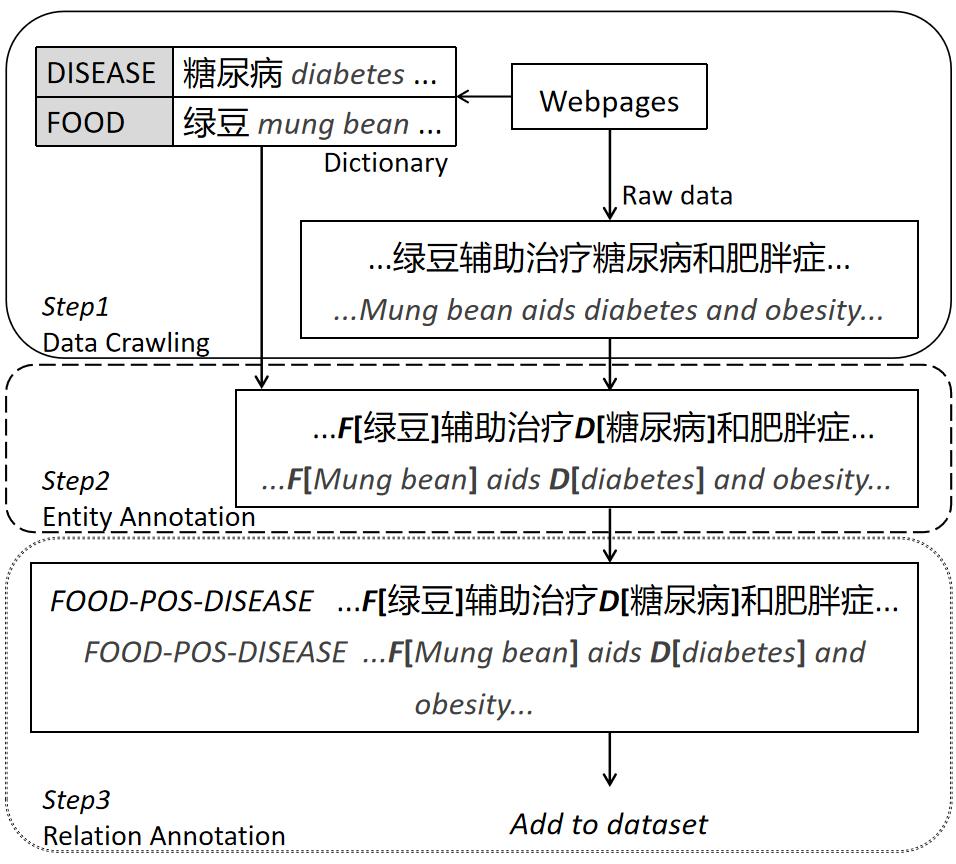
\includegraphics[width=8cm]{datasetconstruct.png}
    \caption{The construction procedure of FRM dataset.}
    \label{fig:construct}
\end{figure}

\subsection{Crawling Corpus and Entity Dictionaries}
The first step of constructing the FRM dataset is to obtain a Chinese medical corpus of considerable size and a dictionary containing different types of entities. Both the corpus and the dictionary is acquired by crawling Chinese health-related websites (\url{http://www.xywy.com},  \url{http://www.39.net} and \url{https://www.9939.com}). An example sentence from the crawled corpus and example entities from dictionaries are shown in Figure \ref{fig:construct} enclosed by the solid rectangle.
\subsection{Auto-labeling Entities}
We automatically align the entities in the dictionary to the sentences in corpus.

We firstly apply longest-exact match to extract sentences that contain two entities in the dictionary. In the longest-exact match procedure, for a candidate string $s$, we denote a substring of length $l$ starting from the $i^{th}$ character as $s_{i,l}$. We adopt a boolean function $m$ where $m(s_{i,l})=True$ if substring $s_{i,l}$ exactly matches an entity in the dictionary, and $False$ otherwise. We go through $s$ from left to right. If $m(s_{i,l})=True$ and there is no $s_{j,k}$ that satisfies (1) $s_{j,k}$ contains $s_{i,l}$ (2)$m(s_{i,l})=True$, we call $s_{i,l}$ a longest matched substring. If a sentence contains two distinct longest matched substrings, we label these two substrings as entities $e$ and add this sentence to a set of candidate sentences.

Then, for each candidate sentence $s$ with entities $e$ labeled, we perform word segmentation on $s$ to split it into words $\{w_0,w_1,...,w_t\}$ where $t$ is the length of the sentence. We assert that for either entity $e_i,i=0,1$ in $e$, it must satisfies $e_i=join(w_j,...w_k)$ for $\forall j,k \in [0...t-1]$ where $join$ is a string joining function. If the requirement is not met, we discard this sentence. Thus only sentences with $e$ that are compete words remain. Example is shown in Figure \ref{fig:construct} the dashed rectangle.
\subsection{Manual Screening and Relation-labeling}
We manually screen out the remaining entity-wrongly-labeled candidate sentences. For each correctly-labeled sentence $s$, we manually tag the relation $r$ to the sentence. Thus we get a triple $(s,e,r)$ and add the triple into the dataset. Example is shown in the dotted rectangle in Figure \ref{fig:construct}.
Relations are manually annotated because of the noise in the crawled sources and the semantic ambiguity issues.
\subsection{Dataset Statistics}


\begin{table}[ht]
\centering
\small
\begin{tabu}{|c|[0.5pt]l|}
\hline
\textbf{Group} & \textbf{Relations} \\ \tabucline[0.5pt]{-}
D-D & complication, cause, is, include, NA \\ \hline
D-S & have, NA\\ \hline
D-F & positive, negative, forbid, prevent, cause, NA\\ \hline
D-N & positive, negative, prevent, lack, cause, NA\\ \hline
F-N & contain, NA\\ \hline
S-F & forbid, cause, positive, negative, prevent, NA\\ \hline
\end{tabu}
\caption{Entity groups in FRM dataset. D,S,F,N stands for Disease, Symptom, Food and Nutrient respectively.}
\label{Egroup}
\end{table}

The FRM dataset contains 27 relations with 50 instances per relation. The 27 relations cover binary relations among 4 entity types. The average length of a sentence in FRM dataset is 67.62, and there are totally 2,187 unique characters.

The 27 relations in FRM dataset can be aggregated into 6 groups according to the entity types (Table \ref{Egroup}). We use separated relations for training and testing. More meaningfully, when treating one group of relations as the test set, other groups serve as the training set. Thus, we can formulate 6 different few-shot relation classification tasks with our FRM dataset.

\begin{table}[ht]
\centering
\small
\begin{tabular}{|l|r|r|r|}
\hline
\textbf{Dataset} & \textbf{\#cls.} & \textbf{\#inst./cls.} & \textbf{\#inst.} \\ \hline
FewRel & 100 & 700 & 70,000 \\ \hline
FRM & 27 & 50 & 1,350 \\ \hline
\end{tabular}
\caption{Comparison of FRM dataset to other few-shot relation classification datasets.}
\label{Datasetcompare}
\end{table}


The FRM dataset provides hard tasks for several reasons. Firstly, we shrink the training data size. Table \ref{Datasetcompare} shows the comparison of data size with previous few-shot relation classification datasets. Secondly, the relations in a given test set are relative to each other since the share common entity types (because the relations are from the same group). In other datasets, the entity types are distinct in most situations, which may serve as extra information. %Figure xx shows example instances from previous datasets and the HEALTHXX dataset. For previous datasets, the instances within the same category is likely to be quite similar while instances from different categories distinct from one to another. While in HEALTHXX datasets, the format of instances within one category varies from one to another, which makes the task harder.

The detailed meaning and example instances of each relation is listed in Appendix ...

\section{Methodology}
In this section, we outline the methodology employed to gather, process, and annotate the data for our study. We begin by detailing the sources of our multimodal video data and personality labels, focusing on how we efficiently align subtitles with original scripts to ensure accurate temporal and character associations. And we also present our annotation process, explaining how we leverage the ChatGPT API to automatically annotate social and emotional relations among characters within the text data. 
\subsection{Source of Data}
Our data source contains mainly two parts, the multimodal video data and personality labels. For video data, we include 14 different genres of TV series and movies via an open-source website\footnote[1]{https://yts.mx/}, and for the scripts and subtitles, we also find other open-source websites\footnote[2]{https://www.simplyscripts.com/}\footnote[3]{https://subscene.com/} for research offering the free scripts and subtitles of many famous movie and television programs. Considering the insufficient labeling method of existing works, we collect the personality annotations from personality database website as well as the voting distribution and align them to correctly scripts. 
\subsection{Data Alignment Process}
As subtitle contain temporal information and original scripts associate utterances with characters, we are supposed to align them properly as efficient as possible. However, most of the existing multimodal datasets annotate the timestamps manually with taking up a great deal of time. There are also some works which utilize different automatic tools to align the utterances with their corresponding information. For instance, \cite{lian2024merbench} use an Automatic Sound Recognition (ASR) tool called Gentle\footnote[4]{https://github.com/lowerquality/gentle} to get the timestamps for the utterances. To streamline the process of aligning dialogue utterances with their respective timestamps and speakers from subtitles, we propose an efficient method leveraging a fuzzy matching algorithm. 
Following successful alignment, we proceed to segment the video content into distinct scenes according to the timestamps. Besides, we use FFmpeg\footnote[5]{https://ffmpeg.org/} to extract the audio track from the video clips and output it as a \textit{.mp3} file.


\begin{figure}[ht]
    \small
    \centering 	 	 	 	
    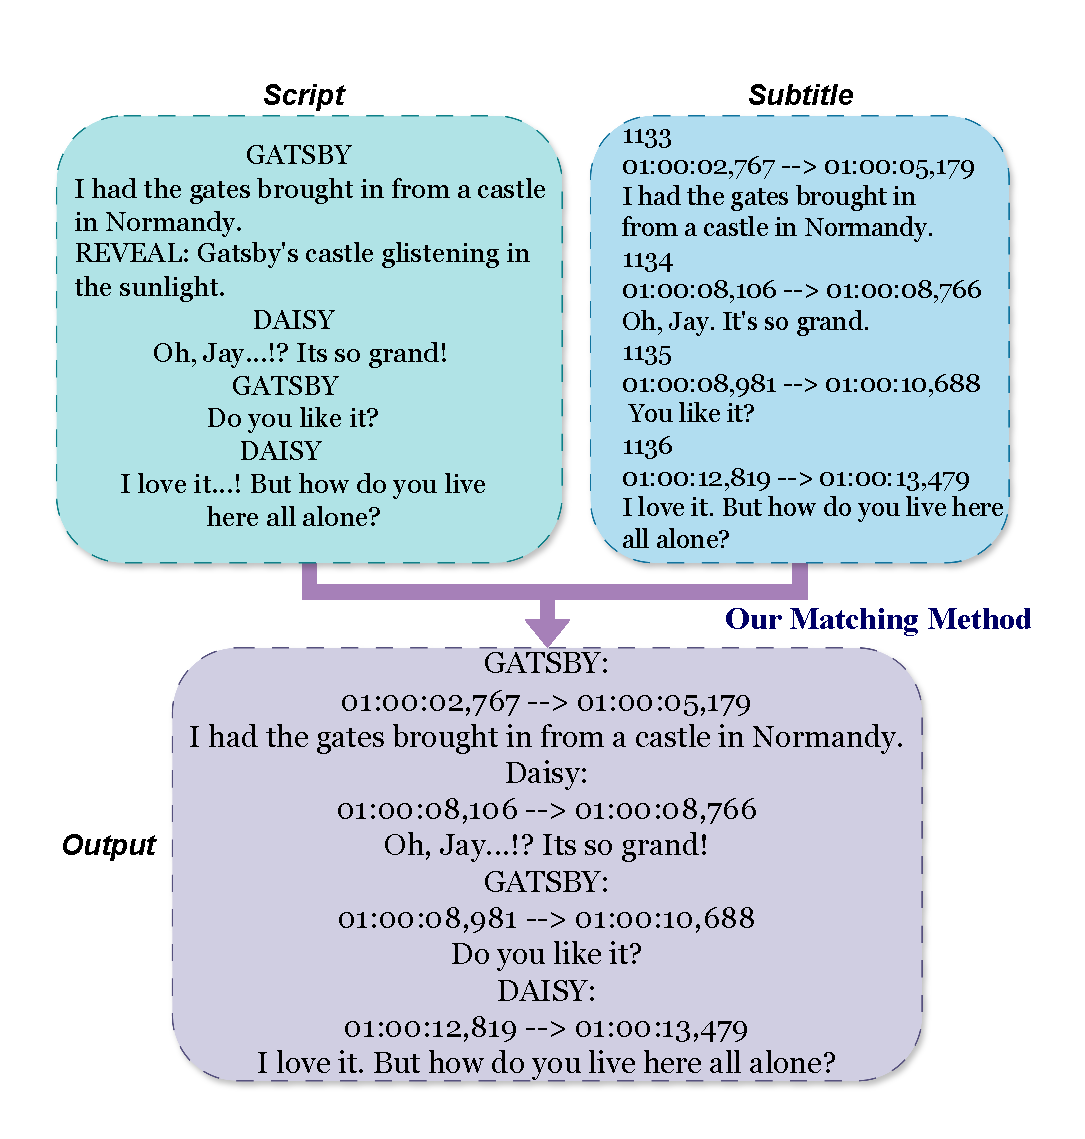
\includegraphics[width=\linewidth, trim= 0 10 0 10, clip]{images/raw_data.pdf}
	\caption{Process of data alignment}
    \label{fig:alig}
\end{figure}

\subsection{Annotation Process}

We developed a process to automatically annotate social and emotional relationships among characters using the ChatGPT API, specifically the \textit{gpt-3.5-turbo-1106} model, which is suited for processing text data. After preprocessing the text and dividing it into scenes, we designed prompts (Fig \ref{fig:prompt}) for ChatGPT to identify social and emotional relationships in each scene. A challenge arose in representing unidirectional affectionate relationships, where one character (A) likes another (B) but the feeling is not mutual. While social relationships are straightforward, emotional relationships require a method to capture this directionality. We addressed this by interpreting the relative position of characters in the tuple: for instance, "A and B (family, fondness)" indicates that A has positive feelings towards B, whereas "B and A (family, fondness)" indicates the opposite. This method effectively captures and represents the directionality of emotional relationships.

\begin{figure}[ht]
	\centering
	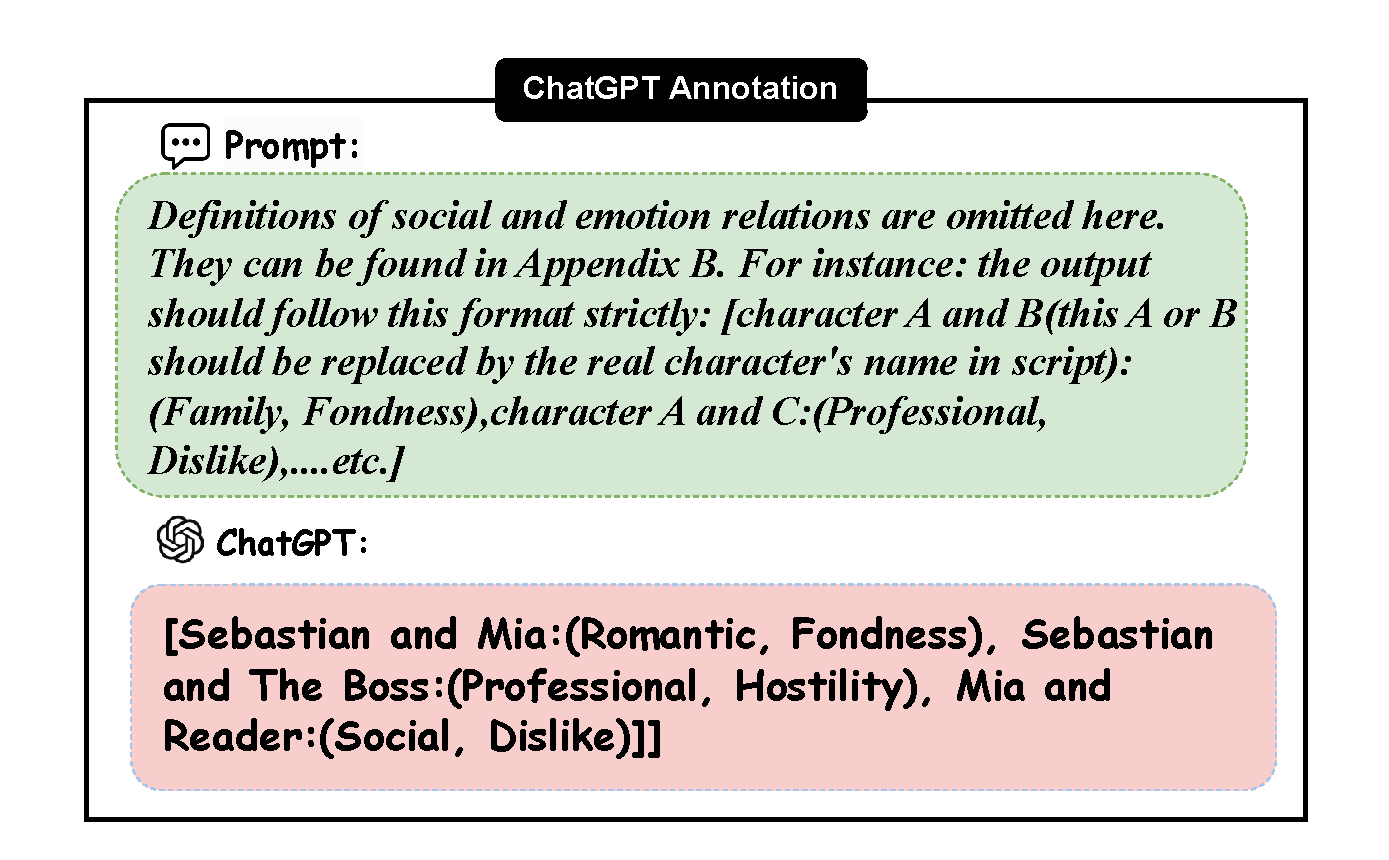
\includegraphics[width=\linewidth]{images/prompt.pdf}
	\caption{Prompt design for relations annotation}
	\label{fig:prompt}
\end{figure}


\section{Evaluation}
 We present the basic statistics of our dataset in the first part, and then we evaluate the accuracy of our alignment and annotation process to ensure their reliability. Additionally, we not only test our dataset on different advanced models but also do ablation experiment on both modality and relations annotation. To discover interesting topics about personality dynamics, we focus on those changes of personality and discover several interesting psychological phenomenons.

\subsection{Dataset Statistics}

As we mentioned before, PersonaMovs is not only a large dataset containing a huge amount of text, audio and video corpus but also its data is highly diverse in terms of personality types, movie and television production genres, and relationship types. Fig \ref{Fig:Relats} are the distribution of two types of relations, which indicates the diversity in terms of interaction scenarios.

\begin{figure}[ht]
    \centering
    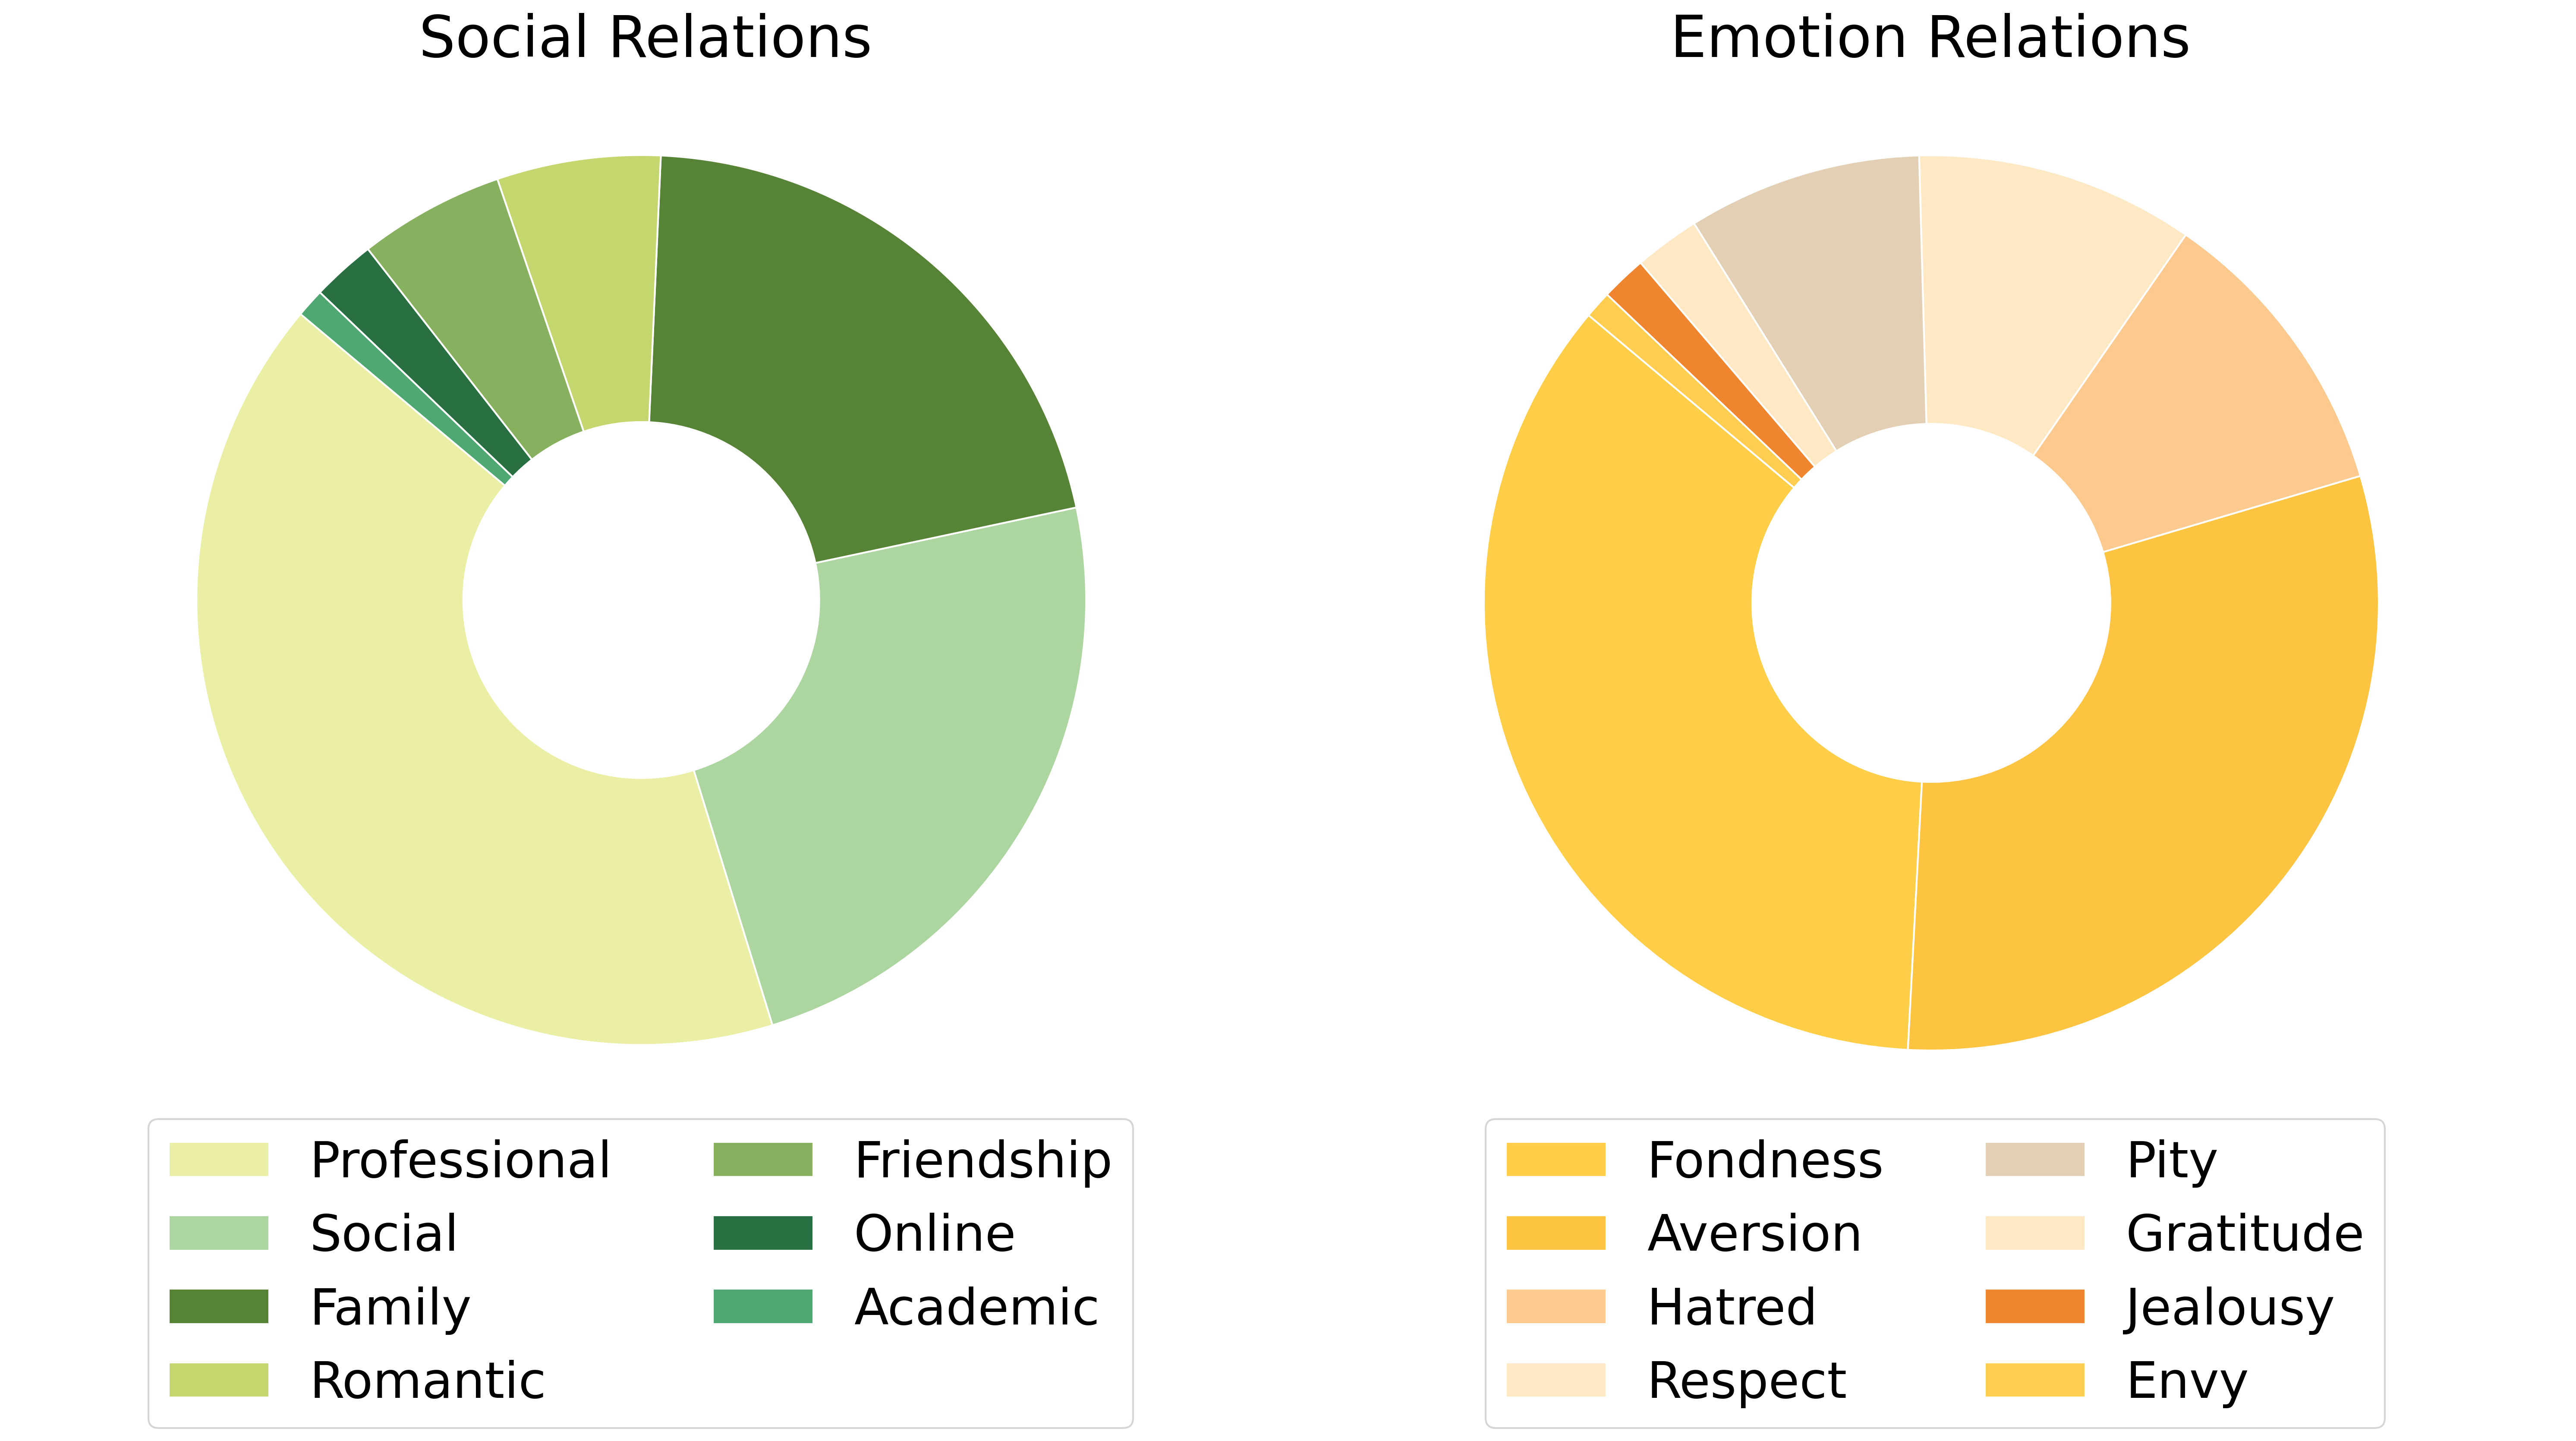
\includegraphics[width=0.75\linewidth]{images/relations.png}
    \caption{Distribution of social and emotion relations}
    \label{Fig:Relats}
\end{figure}


\subsubsection{Algorithm Evaluation}

To evaluate the performance of our character-to-subtitle matching algorithm, we randomly sample a test case comprising over 50 dialogues and 600 utterances from a variety of genres, including 10 films and TV series. We manually check the aligned characters' name based on the script. Our primary metrics for assessment is accuracy. The algorithm demonstrates an accuracy of about 88\%, indicating a high level of accuracy in correctly identifying character names within subtitles across diverse content types. Compared to existing ASR matching algorithm, our approach gains an improvement by 5\% in accuracy. Besides, our algorithm shows a very strong efficiency comparing the ASR method, of which accelerating almost 7 times.

\begin{table}[ht]
    \small
    \centering
    \begin{tabular}{lllc}
        \hline
        \textbf{Method} & \textbf{Movies} & \textbf{TV} & \textbf{Exec. Time (s)}\\
        \hline
        Gentle (ASR) & 82.71\% & 85.21\% & 26.51\\
        \hline
        Our algorithm & 87.53\% & 88.98\% & 3.55\\
        \hline
    \end{tabular}
    \caption{Accuracy and running time per dialogue of subtitle matching algorithm}
\label{table:alg_eval}
\end{table}

\subsubsection{Annotation Accuracy}
Using ChatGPT to annotate relations for the characters is not a completely worthwhile method. To measure the automatic annotation accuracy, we sampled 235 scenes randomly and involved 5 human labelers on relations annotation. These labelers are in their mid-twenties, 
undergraduate or higher education background, proficient in English with majors in psychology, filmography and sociology, who were instructed to select one of the designated social and emotion relations after aligned video. We continue to compare the automatically annotated results to the human-labeled ground truth. The outcome shows that both social and emotional relationship annotations are dependable, with the accuracy reaching 95\% and 84\% respectively.

\begin{table}[ht]
    \centering
    \small
    \begin{tabular}{llll}
        \hline
        \textbf{Task} & \textbf{Movies} & \textbf{TV} & \textbf{Total}\\
        \hline
        Social Relations& 98.21\% & 93.91\% & 95.78\%\\
        \hline
        Emotion Relations& 82.04\% & 84.46\% & 84.01\%\\
        \hline
    \end{tabular}
    \caption{Accuracy of relations annotation.} 
\label{table:annota_eval}
\end{table}

The dataset's foundation on crowdsourced voting allows for an in-depth analysis of subjective biases in personality perception. Researchers can investigate how different demographics (age, gender, cultural background) perceive personality traits and emotions in characters, revealing biases that may exist in personality assessment. This could also extend to studying the impact of viewer's own personality traits on their perceptions of characters, thus contributing to a deeper understanding of projection and identification processes in media consumption.

\subsection{Experiment Results}
\subsubsection{Dataset Difficulties}
We test our dataset on popular models including BERT~\citep{devlin2019bert}, D-DGCN~\citep{yang2023orders}, Roberta~\citep{liu2019roberta}, AttRCNN~\citep{article1}, GPT-3.5~\citep{openai2023gpt35}, GPT-4~\citep{GPT-4-0125} and MCT~\citep{10386376}. Table \ref{table:Method_Comparison} shows the accuracy of our dataset is apparently lower than other competing datasets. One of the main challenges we observed was the complexity and diversity of our dataset compared to other multimedia datasets. 


\begin{table}[ht]
    \centering
    \small
    \begin{tabular}{lllll}
        \hline
        \textbf{Method} & \textbf{Modalities} & \textbf{FP} & \textbf{TVQA} & \textbf{PM} \\
        \hline
        BERT & T only& 61.14 & 60.61 & \textbf{52.94} \\
        \hline
        D-DGCN & T only & 69.56 & 70.21 & \textbf{68.47} \\
        \hline
        Roberta& T only &62.58 & 69.24 & \textbf{60.37} \\
        \hline
        AttRCNN & T only& 65.01 & 67.25 & \textbf{62.44}\\
        \hline
        GPT-3.5 & T only & 69.21 & 66.89 & \textbf{64.08}\\
        \hline
        GPT-4 & T \& V & 79.14 & 78.33 & \textbf{76.90}\\
        \hline
        MCT & T, A \& V & 71.67 & 69.93 & \textbf{68.47} \\
        \hline
    \end{tabular}
    \caption{Accuracy of different methods on Friends Persona (FP), TVQA, and PersonaMovs (PM). T, A, \& V stand for text, audio and video respectively. Lowest accuracy in each row is bolded.} 
\label{table:Method_Comparison}
\end{table}
A more challenging dataset, such as the one we have developed, offers several advantages in terms of personality detection: 1) Our dataset captures a wide range of real-life situations and intricate contexts, which better mirrors the complexity of human interactions. This realism is crucial for developing models that can perform well in practical applications. 2) Training on a more difficult dataset forces models to learn more nuanced patterns and relationships, leading to better generalization capabilities. 3) A difficult dataset sets a high standard for model evaluation, ensuring that only the most effective models are considered successful. This helps in distinguishing truly advanced models from those that perform well only on simpler tasks. Additionally, one notable observation from the results is that the MCT model, which leverages three modalities (text, audio, and video), does not outperform the GPT-4 model, which uses only two modalities (text and video). This performance gap suggests that Large Language Model outperforms the small model on this task, even though the latter uses more modalities.
\subsubsection{The Importance of Multi-Modality}
\begin{figure*}[ht]
    \centering
    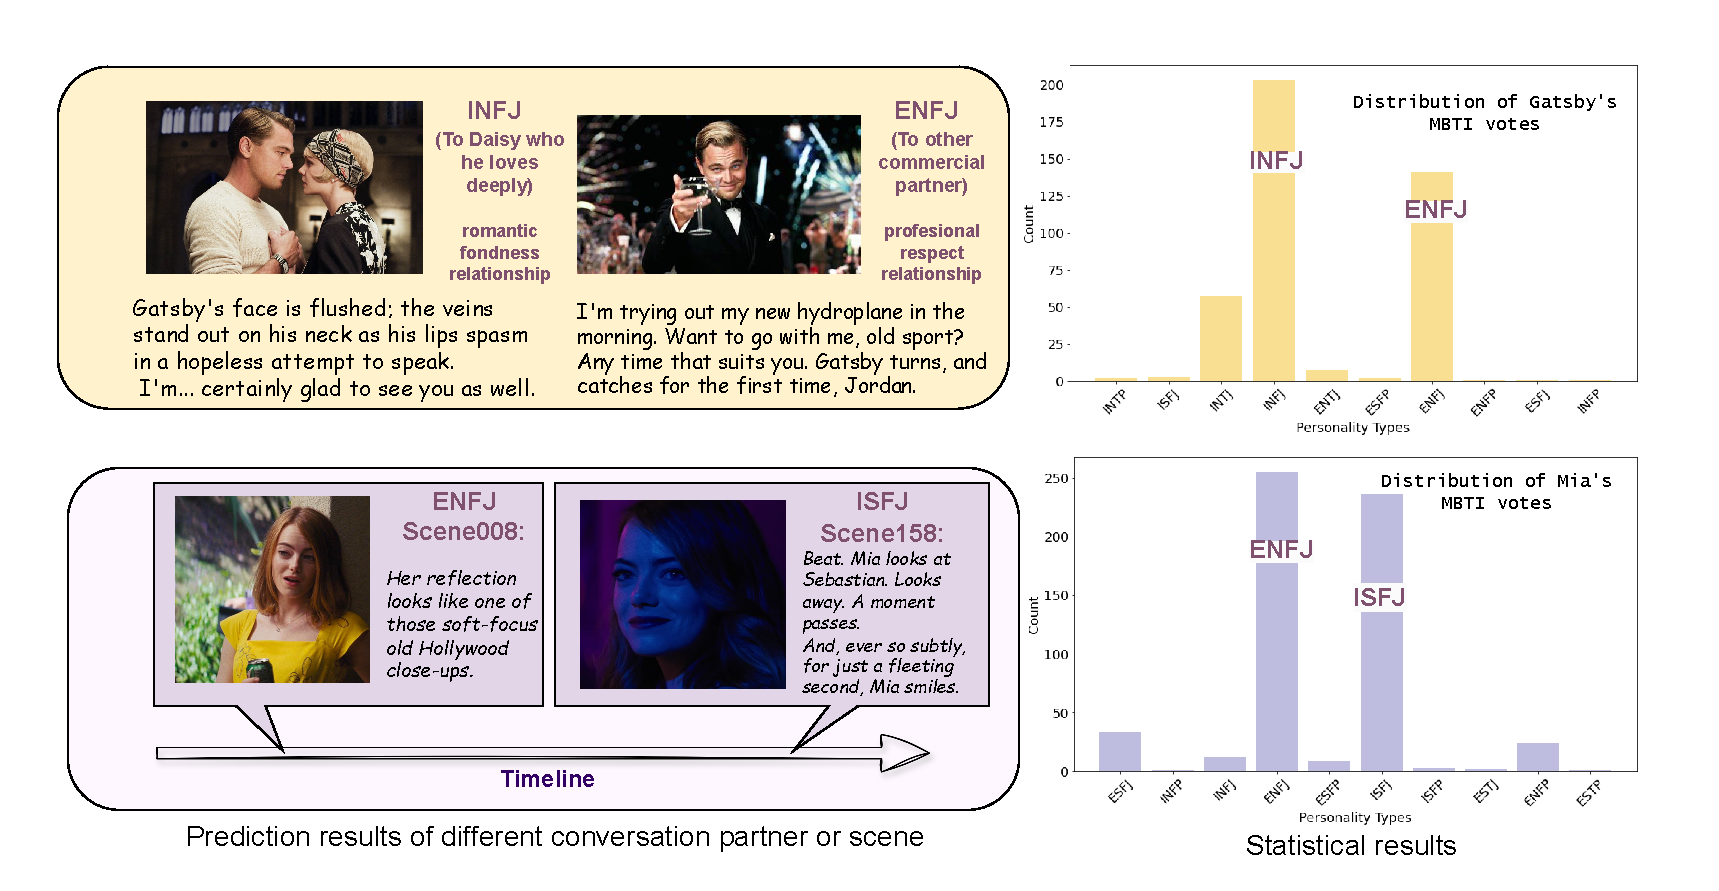
\includegraphics[width=\textwidth, trim= 0 10 0 0, clip]{images/Dynamics.pdf}
    \caption{Case study for personality dynamics.}
    \label{fig:dynamics}
\end{figure*}


We conducted a series of ablation experiments to assess the impact of different modalities and relations annotations on the performance of personality prediction models. The experiments were designed to understand how the exclusion of specific modalities or relations annotations affects the overall prediction accuracy.

\begin{table}[ht]
    \small
    \centering
    \begin{tabular}{c|c|c}
        \hline
        \textbf{Method} & \textbf{Modality} & \textbf{Accuracy}\\
        \hline
        \multirow{4}{*}{MCT} & T \& A & 66.13  \\
        & T \& V & 67.91 \\
        & T only & 63.43 \\
        & T, A \& V & 68.47 \\  
        \hline
        \multirow{2}{*}{GPT-4-0125} & T only & 70.20 \\     
        & T \& V & 76.90 \\
        \hline
    \end{tabular}
    \caption{Ablation experiment on different modalities} 
\label{table:Ablation_modal}
\end{table}


Table \ref{table:Ablation_modal} presents the results of ablation experiments where different combinations of video and audio modalities were excluded. The result underscore the critical importance of using multiple modalities to achieve higher accuracy in personality prediction tasks. Models that leverage both audio and video data, in addition to text, consistently outperform those that rely solely on textual data. 
\begin{table}[ht]
    \centering
    \small
    \begin{tabular}{ccc}
        \hline
        \textbf{Method} & \textbf{With Relations} & \textbf{Without Relations} \\
        \hline
        BERT & 53.88 & 52.94 \\
        \hline
        Roberta & 59.21 & 58.39 \\
        \hline
        GPT-4-0125 & 73.22 & 70.20 \\  
        \hline
    \end{tabular}
    \caption{Ablation experiment on relations annotations.}
    \label{table:Ablation_relationship}
\end{table}

Table \ref{table:Ablation_relationship} shows the results of ablation experiments focusing on the inclusion or exclusion of relations' annotations which finds the relations annotations tend to slightly enhance the performance. This highlights the importance of including rich contextual information to improve the accuracy of personality prediction models. 


The multimodal nature of the dataset (incorporating video, audio, textual, and crowd-sourced data) enables comprehensive studies that integrate different data types to understand personality. This could lead to the development of new theories or the refinement of existing ones that account for the complexity of personality as depicted through various media. It could also foster interdisciplinary research, combining insights from psychology, computer science, linguistics, and media studies.
\subsubsection{Personality Dynamics}

Movies and TV series and their characters often evolve over time, offering a fertile ground for studying personality dynamics. The dataset allows for longitudinal studies on how characters' personalities change in response to narrative events, relationships, and challenges. This could lead to new models that explain personality development and dynamics in complex social settings, bridging narrative theory and psychological research. 

We manually select two famous characters to find their potential change of personality, and we discover there are two types of personality shifts. In the short term, people show different personalities depending on their relations with interlocutor. For example, as shown in Figure \ref{fig:dynamics}, Jay Gatsby from the famous romantic movie called ``\textit{The Great Gatsby}'' behaves as an INFJ in front of his beloved Daisy and as an ENFJ in front of his business partners. In the long term, people may change their personality due to major turning point of life. Like Mia Dolan in ``\textit{La La Land}'', she was always ENFJ, but after the breakup she became an ISFJ. The prediction results generated by GPT-4 align with the peaks in the voting distribution, indicating that this personality shift is observable within our realistic dataset.

According to our finding, we conduct statistical analysis based on our dataset to figure out if there exists certain personalities that are easily attracted to each other. To analyze the patterns of personality attraction, we focus on identifying pairs of personalities that frequently appear together bi-directionally in fondness, aversion, romantic and friendship relations. Figure \ref{fig:networks} presents the favorite network with 16 MBTI personality types, providing a clear visual summary of statistical findings. The size of each node is proportional to the number of connections (degree) it has, which means personality types with more relationships are represented by larger nodes. The color of the edges represents the weight of the relationship between the personality types. Darker edges indicate a higher frequency or stronger relationship. 
%Based on these vivid figures, we can discover very interesting psychological phenomenons. 
For instance, ISTP is the most popular personality since almost every other personality has a fondness relation with it, and ESTP prefers to be around ESFP, ENFP and people with the same personality as themselves. ESFP may not like people with same personality.
% because it has a dark circle on itself.


\begin{figure}[!h]
    \centering
    \begin{subfigure}[b]{0.22\textwidth} 
        \centering
        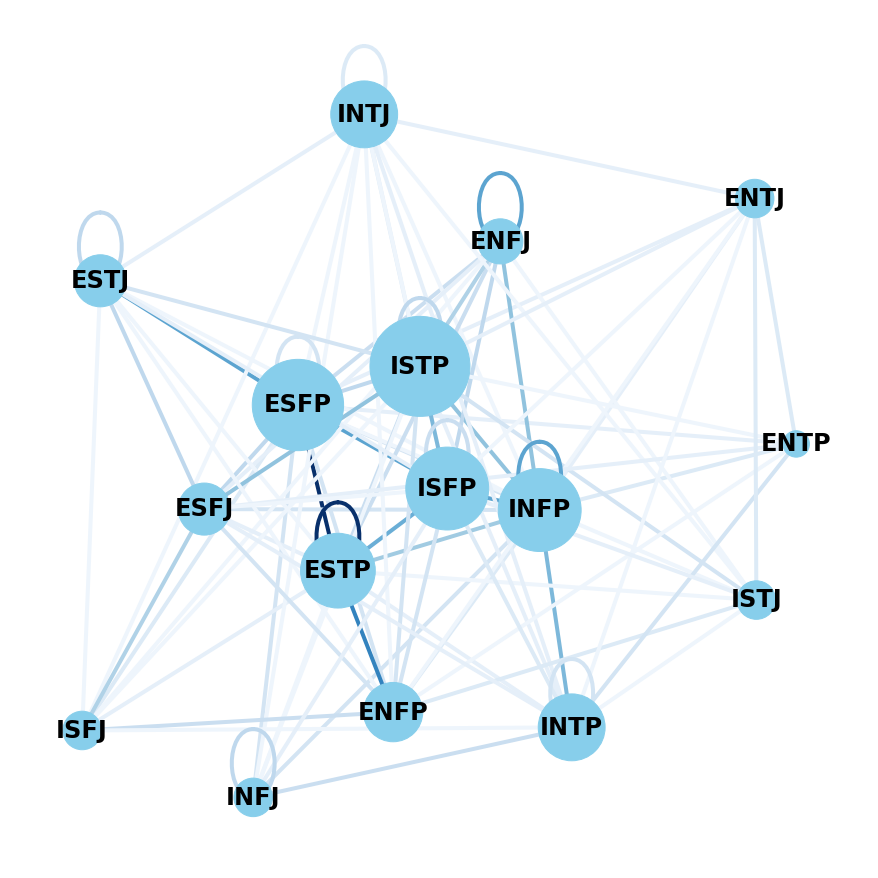
\includegraphics[width=\linewidth, scale=0.7]{images/fondness.png} 
        \caption{Fondness}
        \label{fig:subgraph1}
    \end{subfigure}
    \hfill
    \begin{subfigure}[b]{0.22\textwidth} 
        \centering
        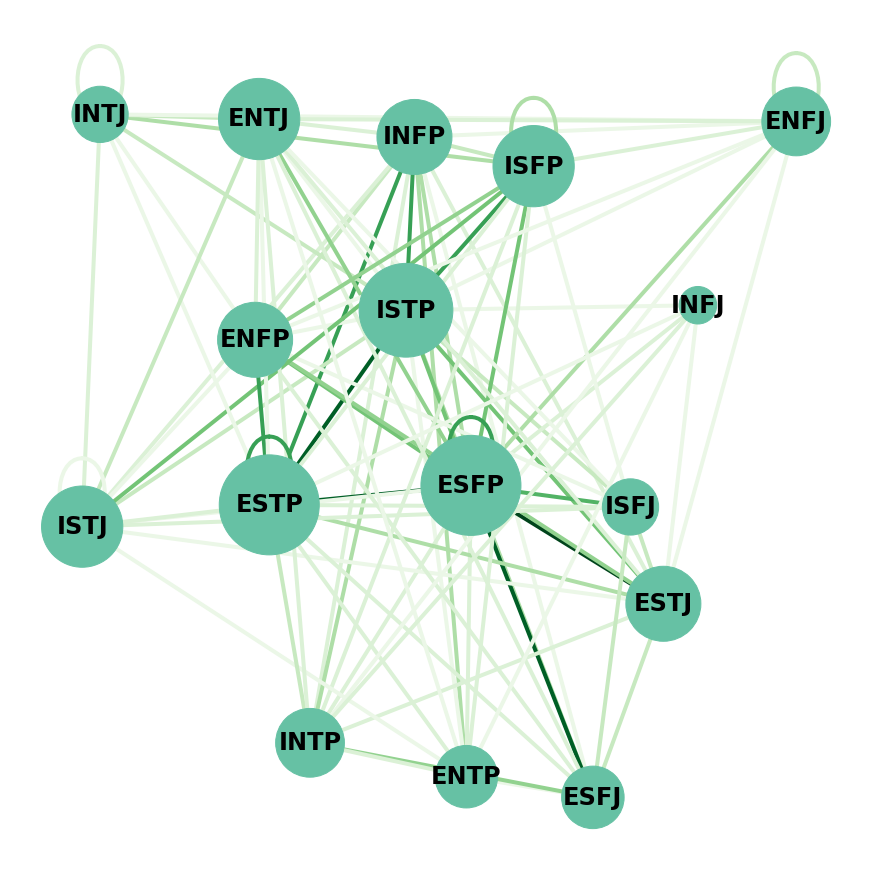
\includegraphics[width=\linewidth, scale=0.7]{images/dislike.png}
        \caption{Aversion}
        \label{fig:subgraph2}
    \end{subfigure}
    \hfill
    \begin{subfigure}[b]{0.22\textwidth} 
        \centering
        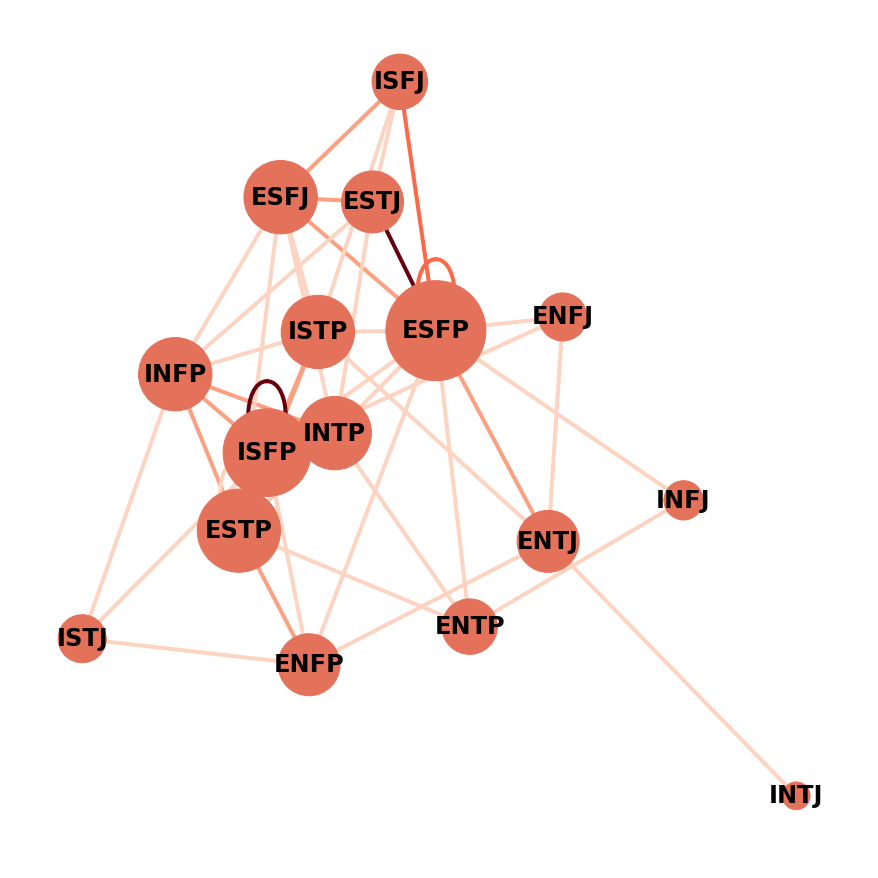
\includegraphics[width=\linewidth, scale=0.7]{images/romantic.png}
        \caption{Romantic}
        \label{fig:subgraph3}
    \end{subfigure}
    \hfill
    \begin{subfigure}[b]{0.22\textwidth} 
        \centering
        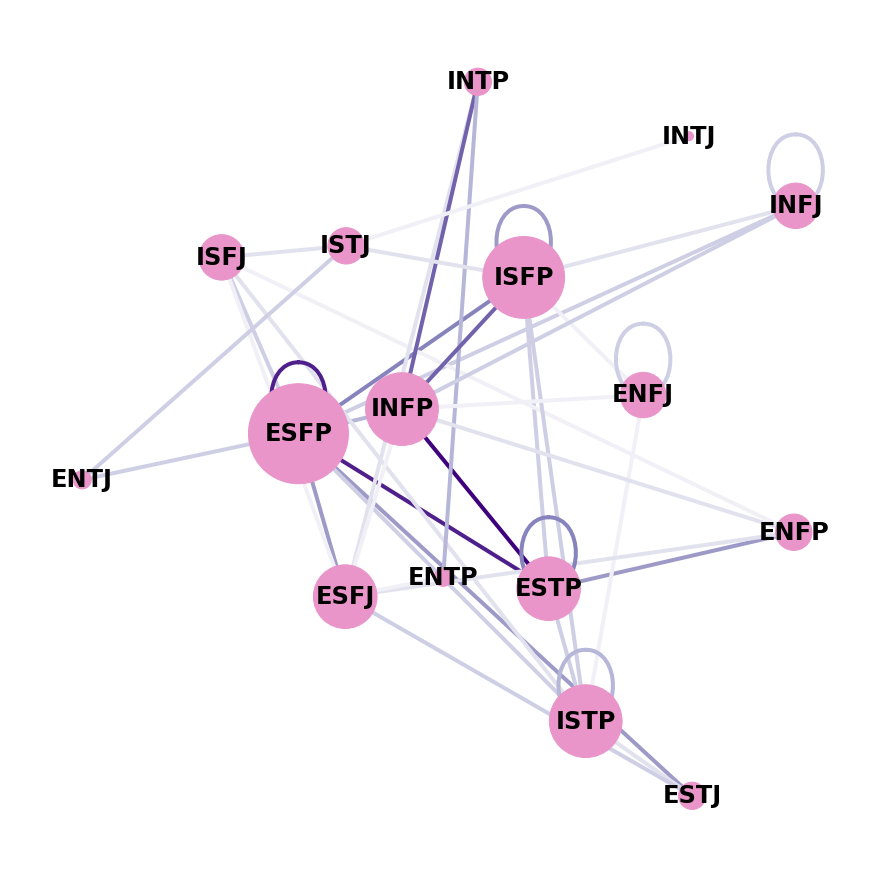
\includegraphics[width=\linewidth, scale=0.7]{images/friendship.png} 
        \caption{Friendship}
        \label{fig:subgraph4}
    \end{subfigure}
    \caption{Favorite Networks with Different Personalities about Four Relations}
    \label{fig:networks}
\end{figure}

By including data on social and emotion relations between characters, the dataset opens new pathways for exploring the dynamics of personality through interactions. This aspect can support research into how different personality types influence and are influenced by social networks, both within narrative contexts and long-term conversions. It provides a basis for computational models that simulate personality dynamics in social networks, potentially informing theories on social behavior, conflict resolution, and group dynamics.

\section{Conclusion}

In this study, we conducted a comprehensive analysis of Prison Term Prediction (PTP) and identified two major issues: structural representation of legal knowledge and the scarcity of training data for most crimes. To address these issues, we proposed a novel approach, \lawgraph{}, to represent the structural legal knowledge. We further proposed a lightweight Statute Knowledge Encoder (SKE) for end-to-end training of our model. We performed extensive experiments to compare SKE with previous works and LLMs. The experimental results have indicated the superiority of SKE over previous works. 

\section*{Ethical Statements}

Copyright © [2024] by the authors. The movies and TV series included in this dataset are copyrighted by their respective copyright owners and are used in this work for academic and research purposes under fair use guidelines or specific permissions obtained from the copyright holders. This does not imply endorsement by or affiliation with the copyright owners. Use of these materials is limited to the scope of the permission granted and is not intended for commercial distribution.


\section{Limitation}

Our framework is a two-phase process, which has its inherent defects, that is, the results of the second phase depend on the results of the first phase. Because the sequence annotation algorithm in the first phase cannot achieve 100\% accuracy, it will predict the wrong position that should be rewritten when the second phase is followed, which will further lead to the error of the final result.

On the other hand, T5 model is only used to predict the words that should be filled in blank, rather than generate the whole sentence, which may lead to the decline of the overall fluency of the sentence.


\bibliography{custom}

\appendix
\section{Definitions of Personality Models}
\label{sec:appendixA}

\begin{itemize}
  \item \textbf{Myers–Briggs Type Indicator (MBTI)}: The MBTI categorizes personality into four dimensions. Extraversion (E) vs. Introversion (I): Extraverts are outgoing and energized by social interactions, while Introverts are reserved and energized by solitude. Sensing (S) vs. Intuition (N): Sensors focus on present, concrete information, valuing practicality, whereas Intuitives are imaginative and future-oriented, valuing abstract ideas. Thinking (T) vs. Feeling (F): Thinkers base decisions on logic and fairness, prioritizing objectivity, while Feelers base decisions on personal values and the impact on others, prioritizing harmony. Judging (J) vs. Perceiving (P): Judgers prefer structured and organized lives, liking plans and decisiveness, while Perceivers prefer flexibility and spontaneity, liking to keep their options open. Each MBTI type is defined by a combination of four cognitive functions, which can be either introverted (i) or extraverted (e). Extraverted Sensing (Se): Focuses on the present moment and physical reality, highly attuned to sensory experiences. Introverted Sensing (Si): Relies on past experiences and memories, valuing tradition and consistency. Extraverted Intuition (Ne): Sees patterns and connections, focusing on future possibilities and abstract ideas. Introverted Intuition (Ni): Focuses on internal insights and foresight, seeing underlying meanings and future potentials. Extraverted Thinking (Te): Organizes and structures the external world, prioritizing logic and efficiency. Introverted Thinking (Ti): Analyzes and categorizes information internally, valuing logical consistency and understanding. Extraverted Feeling (Fe): Prioritizes harmony and social values, focusing on the needs and feelings of others. Introverted Feeling (Fi): Values personal beliefs and feelings, making decisions based on inner values and ethics.
  \begin{table*}[ht]
    \centering
    \small
    \begin{tabular}{ll}
      \hline
      \textbf{Relations type} & \textbf{Description}\\
      \hline
      Family & Parents (grandparents) and children, siblings, etc.\\
      \hline
      Friendship & Based on common interest, mutual respect and affection, but not related to the blood.\\
      \hline
      Romantic & Based on emotional attraction and include dating, marriage, etc.\\
      \hline
      Professional & Formed in a work environment, such as colleagues, superiors and subordinates, etc.\\ 
      \hline
      Social & Formed in a broader social context, such as neighbors, club members.\\
      \hline
      Academic & Formed in an educational setting, such as between teachers and students, classmates.\\
      \hline
      Online & Established in online spaces or through social media platforms.\\
      \hline
    \end{tabular}
    \caption{Descriptions of Social Relations}
    \label{table:social}
    \end{table*}
    
    \begin{table*}[ht]
      \small
      \centering
      \begin{tabular}{ll}
        \hline
        \textbf{Relations type} & \textbf{Description}\\
        \hline
        Fondness & A positive emotion characterized by a person's fondness for another.\\
        \hline
        Jealousy & Unhappy and angry because someone has something that you want.\\
        \hline
        Aversion  & A negative emotion, referring to a feeling of disfavor towards someone.\\
        \hline
        Pity  & A feeling of sadness for someone else's difficult situation.\\ 
        \hline
        Respect & Admiration felt or shown for someone that you believe has good ideas or qualities.\\
        \hline
        Hostility  & An unfriendly or unkindness towards someone or something.\\
        \hline
        Envy & A discontented feeling when a person desires what someone else has.\\
        \hline
        Gratitude & An emotion of being thankful for someone else's help or kind actions.\\
        \hline
      \end{tabular}
      \caption{Description of Emotion Relations}
      \label{table:emotional}  
    \end{table*}
  \item \textbf{Big Five Personality Traits}: The Big Five model describes personality using five broad traits. Openness to Experience: High openness involves imagination and insight, while low openness involves practicality and routine. Conscientiousness: High conscientiousness is characterized by organization and dependability, while low conscientiousness is characterized by spontaneity and flexibility. Extraversion: High extraversion includes sociability and assertiveness, while low extraversion (introversion) includes reserve and solitude. Agreeableness: High agreeableness involves trust and altruism, while low agreeableness involves skepticism and competition. Neuroticism: High neuroticism involves emotional instability and anxiety, while low neuroticism involves emotional stability and calmness.
  \item \textbf{Enneagram}: The Enneagram classifies personality into nine types, each representing different motivations and fears. Type 1: The Reformer, driven by a need for perfection. Type 2: The Helper, driven by a need to be loved. Type 3: The Achiever, driven by a need for success. Type 4: The Individualist, driven by a need for uniqueness. Type 5: The Investigator, driven by a need for knowledge. Type 6: The Loyalist, driven by a need for security. Type 7: The Enthusiast, driven by a need for variety and fun. Type 8: The Challenger, driven by a need for control. Type 9: The Peacemaker, driven by a need for harmony. A 2w3 individual is likely to be more ambitious, charming, and goal-oriented than a typical Type 2. They still seek to help others but are also motivated by a desire for success and recognition.
  \item \textbf{Instinctual Variants}: The Instinctual Variants theory describes three primary instinctual drives influencing behavior. Self-Preservation (SP): Focuses on safety, health, and comfort. Social (SO): Focuses on relationships, status, and community. Sexual (SX): Focuses on intimacy, attraction, and one-on-one connections. For instance, an 8w7 with a Sexual variant, is highly charismatic and seeks intense and passionate connections with others. He or she is bold and assertive, often focusing his or her energy on building strong, impactful relationships.
\end{itemize}

\section{Definitions of Relations}
\label{sec:appendixB}
Human social networks are complex and multifaceted. By categorizing relations, we can better understand the dynamics and nuances of how people interact with each other. Different types of relations provide context for interactions, which is crucial for analyzing social behaviors and patterns, improving social network analysis, and applying this knowledge across various fields and applications.
Table \ref{table:social} and Table \ref{table:emotional} provide a structured approach to understanding the complex web of relations that individuals navigate. By categorizing these relations into social and emotional types, we can better analyze and predict personality dynamics in various contexts~\citep{Collins_Sroufe_1999, 10.1093/acprof:oso/9780195150100.001.0001}. 



\section{Data Alignment Algorithm}
\label{sec:appendixC}
The details of data alignment algorithm are as follows:
\begin{algorithm}[!h]
	\small
	\caption{Scripts and Subtitles Matching}
	\label{alg:Matching}
	\renewcommand{\algorithmicrequire}{\textbf{Input:}}
	\renewcommand{\algorithmicensure}{\textbf{Output:}}
	
	\begin{algorithmic}[1]
		\REQUIRE $Script, Subtitles$
		\ENSURE Updated subtitles with speaker names
		\STATE $dial \& speakers \gets empty$
		\STATE $threshold \gets 0.8$
		\FOR{$scene$ in $Script$}
		\FOR{$Dials$ in $scene$}
		\STATE Extract $speaker$ and $dial$ from $Dials$
		\STATE $dial \& speakers \gets speaker, dial$ 
		\ENDFOR
		\ENDFOR
		\FOR{$subtitle$ in $Subtitles$}
		\STATE $match\_score \gets 0$
		\STATE $match\_speaker \gets Null$
		\FOR{$line$ in $subtitle$}
		\FOR{$speaker, dial$ in $dial \& speakers$}
		\STATE $score \gets Similar(subtitle, dial)$
		\IF{$score$ > $match\_score$}
		\STATE Update $match\_score$ and $match\_speaker$
		\ENDIF
		\ENDFOR
		\IF{$match\_score \geq threshold$}
		\STATE Update $line$ with $match\_speaker$
		\ENDIF
		\ENDFOR
		\STATE Update $subtitle$
		\ENDFOR
		\RETURN Updated $Subtitles$
	\end{algorithmic}
\end{algorithm}

\begin{enumerate}
      \item \textit{Preprocess the raw data} Firstly, we divide the scripts into several scenes according to the coherence in language of camera, instead of randomly clipping in a certain time period. This segmentation is guided by explicit scene transition cues found in movie scripts, such as ``\textit{CUT TO:}'' or scene location indicators. For TV show scripts, which might lack uniform scene transition markers, we identify scene changes by detecting pauses exceeding 3 seconds between utterances.
      \item \textit{Match the utterance} This algorithm is rooted in the comparison of utterances from original scripts and subtitles based on a similarity threshold. If the similarity between a pair of utterances meets or exceeds this threshold, the character's name is accurately associated with the utterance.
      \item \textit{Rematch with the slide window} Basically, the content in scripts is slightly different with the subtitles, because the director may have improvised on the set. Thus, we introduce a slide window algorithm to evaluate the utterance-level similarity. As shown in Algorithm \ref{alg:window}, we set a window to slide over the script and, for each utterance, compare the content inside the window with each subtitle entry to get the similarity of the paragraph in the window. 
\end{enumerate}

\begin{algorithm}[h]
	\caption{Slide Window Matching}
	\small
	\label{alg:window}
	\renewcommand{\algorithmicrequire}{\textbf{Input:}}
	\renewcommand{\algorithmicensure}{\textbf{Output:}}
	
	\begin{algorithmic}[1]
		\REQUIRE $Script, Subtitles$
		\ENSURE Updated subtitles 
		\STATE $window\_size \gets 10$
		\STATE $threshold \gets 0.8$
		\STATE $matches \gets empty\_list$
		\FOR{$i \gets 0$ to $Len(Script) - window\_size$}
		\STATE $window \gets slice(scriptTokens, i, i + window\_size)$
		\STATE $match\_score \gets 0$
		\FOR{$j \gets 0$ to $Len(Subtitles) - 1$}
		\STATE $score \gets Similar(window, Subtitles[j])$
		\IF{$score$ > $match\_score$}
		\STATE Update $match\_score$
		\ENDIF
		\ENDFOR
		\IF{ $match\_score \geq threshold$}
		\STATE $matches \gets Subtitles[j]$
		\ENDIF
		\ENDFOR
		\RETURN Updated $Subtitles$ with $matches$
	\end{algorithmic}
\end{algorithm}

%\section{Prompt Design}
%\label{appedix:prompt}

\end{document}
